% presentation
\documentclass{beamer}
\usetheme[height=7mm]{Rochester}
\usecolortheme{rose}

% handout

%\documentclass[handout]{beamer}
%\usepackage{pgfpages} \pgfpagesuselayout{8 on 1}[a4paper]

%\documentclass[mathserif]{article}
%\usepackage{beamerarticle}

\usepackage{amsmath}
\usepackage{comment}
\usepackage{amssymb,amsfonts}
\usepackage[T1]{fontenc}
\usepackage{lmodern}
\usepackage{tikz}
\usepackage{simpsons}
\usepackage{marvosym}
\usepackage{color}
\usepackage{multirow}
\usepackage{pgffor}
\usepackage[slide,algoruled,titlenumbered,vlined,noend,linesnumbered,]{algorithm2e}

\usefonttheme{structurebold}

\setbeamertemplate{footline}[frame number]
\setbeamertemplate{navigation symbols}{}
\setbeamerfont{smallverb}{size*={73}}
\usefonttheme[onlymath]{serif}
\setbeamertemplate{theorems}[numbered]
\newtheorem{construction}[theorem]{Construction}
\newtheorem{proposition}[theorem]{Proposition}

\AtBeginSection[] {
  \begin{frame}
    \frametitle{Content}
    \tableofcontents[currentsection]
  \end{frame}
  \addtocounter{framenumber}{-1}
}

\usetikzlibrary[shapes.arrows]
\usetikzlibrary{shapes.geometric}
\usetikzlibrary{backgrounds}
\usetikzlibrary{positioning}
\usetikzlibrary{calc}
\usetikzlibrary{intersections}
\usetikzlibrary{fadings}
\usetikzlibrary{decorations.footprints}
\usetikzlibrary{patterns}
\usetikzlibrary{shapes.callouts}
\usetikzlibrary{fit}
%handout

\providecommand{\abs}[1]{\lvert#1\rvert}

\tikzset{every picture/.style={line width=1pt,show background rectangle},background rectangle/.style={fill=blue!10,rounded corners=2ex}}

\author{Yu Zhang}
\institute{Harbin Institute of Technology}
\date[Crypto'20A]{Cryptography, Autumn, 2020}

%% presentation
\documentclass{beamer}
\usetheme[height=7mm]{Rochester}
\usecolortheme{rose}

% handout

%\documentclass[handout]{beamer}
%\usepackage{pgfpages} \pgfpagesuselayout{8 on 1}[a4paper]

%\documentclass[mathserif]{article}
%\usepackage{beamerarticle}

\usepackage{amsmath}
\usepackage{comment}
\usepackage{amssymb,amsfonts}
\usepackage[T1]{fontenc}
\usepackage{lmodern}
\usepackage{tikz}
\usepackage{simpsons}
\usepackage{marvosym}
\usepackage{color}
\usepackage{multirow}
\usepackage{pgffor}
\usepackage[slide,algoruled,titlenumbered,vlined,noend,linesnumbered,]{algorithm2e}

\usefonttheme{structurebold}

\setbeamertemplate{footline}[frame number]
\setbeamertemplate{navigation symbols}{}
\setbeamerfont{smallverb}{size*={73}}
\usefonttheme[onlymath]{serif}
\setbeamertemplate{theorems}[numbered]
\newtheorem{construction}[theorem]{Construction}
\newtheorem{proposition}[theorem]{Proposition}

\AtBeginSection[] {
  \begin{frame}
    \frametitle{Content}
    \tableofcontents[currentsection]
  \end{frame}
  \addtocounter{framenumber}{-1}
}

\usetikzlibrary[shapes.arrows]
\usetikzlibrary{shapes.geometric}
\usetikzlibrary{backgrounds}
\usetikzlibrary{positioning}
\usetikzlibrary{calc}
\usetikzlibrary{intersections}
\usetikzlibrary{fadings}
\usetikzlibrary{decorations.footprints}
\usetikzlibrary{patterns}
\usetikzlibrary{shapes.callouts}
\usetikzlibrary{fit}
%handout

\providecommand{\abs}[1]{\lvert#1\rvert}

\tikzset{every picture/.style={line width=1pt,show background rectangle},background rectangle/.style={fill=blue!10,rounded corners=2ex}}

\author{Yu Zhang}
\institute{Harbin Institute of Technology}
\date[Crypto'20A]{Cryptography, Autumn, 2020}

%\input{1introduction.tex}
%\input{2perfectlysecret.tex}
%\input{3privatekey.tex}


\title{Introduction}

\begin{document}
\maketitle
\begin{frame}
\frametitle{Outline}
\tableofcontents
\end{frame}
\section{Cryptography and Modern Cryptography}
\begin{frame}\frametitle{What is Cryptography?}
\begin{itemize}
\item \textbf{Cryptography}: from Greek \emph{krypt\'os}, ``hidden, secret''; and \emph{gr\'{a}phin}, ``writing''
\item \textbf{Cryptography}: the art of writing or solving codes.\\ (Concise oxford dictionary 2006)
\item \textbf{Codes}: a system of prearranged signals, especially used to ensure secrecy in transmitting messages. \\ (\emph{code word} in cryptography)
\item \textbf{1980s}: from Classic to Modern; from Military to Everyone
\item \textbf{Modern cryptography}: the scientific study of mathematical techniques for securing digital information, systems, and distributed computations against adversarial attacks
\end{itemize}
\end{frame}
\section{The Setting of Private-Key Encryption}
\begin{frame}\frametitle{Private-Key Encryption}
\begin{itemize}
\item \textbf{Goal}: to construct \textbf{ciphers} (encryption schemes) for providing secret communication between two parties sharing \textbf{private-key} (the symmetric-key) in advance
\item \textbf{Implicit assumption}: there is some way of initially sharing a key in a secret manner
\item \textbf{Disk encryption}: the same user at different points in time
\end{itemize}
\end{frame}
\begin{frame}\frametitle{The Syntax of Encryption}
\begin{figure}
\begin{center}
\begin{tikzpicture}
\node (sender) [minimum size=1cm] {}; \Alice{0}{0}{0.4};
\node (bart) [below of = sender, node distance = 0.7cm] {Alice};
\node (enc) [draw, right of = sender, rounded corners=1ex,node distance = 2cm] {$\mathsf{Enc}$};
\node (k1) [above of = enc, node distance = 1cm] {$k$};
\node (c) [right of = enc, node distance = 2cm] {$c$};
\node (gen) [draw, above of = c, rounded corners=1ex,node distance = 1cm] {$\mathsf{Gen}$};
\node (adv) [below of = c, node distance = 1cm, minimum size=1cm] {}; \Evil{4cm}{-1cm}{0.4};
\node (burns) [below of = adv, node distance = 0.7cm] {Adversary};
\node (dec) [draw, right of = c, rounded corners=1ex,node distance = 2cm] {$\mathsf{Dec}$};
\node (k2) [above of = dec, node distance = 1cm] {$k$};
\node (receiver) [right of = dec, node distance = 2cm, minimum size=1cm] {}; \Bob{8cm}{0}{0.4};
\node (lisa) [below of = receiver, node distance = 0.7cm] {Bob};
\draw[-latex] (sender) -- (enc) node [midway, above] {$m$};
\draw (enc) -- (c); \draw[-latex] (c) -- (dec);
\draw[-latex] (dec) -- (receiver) node [midway, above] {$m$};
\draw[-latex] (k1) -- (enc);
\draw[-latex] (gen) -- (k1);
\draw[-latex] (gen) -- (k2);								
\draw[-latex] (k2) -- (dec);		
\end{tikzpicture}
\end{center}
\end{figure}
\begin{itemize}
\item key $k \in \mathcal{K}$, plaintext (or message) $m \in \mathcal{M}$, ciphertext $c \in \mathcal{C}$
\item \textbf{Key-generation} algorithm~$k \gets \mathsf{Gen}$
\item \textbf{Encryption} algorithm~$c:= \mathsf{Enc}_k(m)$
\item \textbf{Decryption} algorithm~$m:= \mathsf{Dec}_k(c)$
\item \textbf{Encryption scheme}: $\Pi = (\mathsf{Gen}, \mathsf{Enc}, \mathsf{Dec})$
\item \textbf{Basic correctness requirement}: $\mathsf{Dec}_k(\mathsf{Enc}_k(m)) = m$
\end{itemize}
\end{frame}
\begin{frame}\frametitle{Securing Key vs Obscuring Algorithm}
\begin{itemize}
\item Easier to maintain secrecy of a short key
\item In case the key is exposed, easier for the honest parties to change the key
\item In case many pairs of people, easier to use the same algorithm, but different keys
\end{itemize}
\begin{alertblock}{Kerckhoffs's principle}
\begin{quote}
The cipher method must not be required to be secret, and it must be able to fall into the hands of the enemy without inconvenience.
\end{quote}	
\end{alertblock}
\end{frame}
\begin{frame}\frametitle{Why ``Open Cryptographic Design''}
\begin{itemize}
\item Published designs undergo public scrutiny are to be stronger
\item Better for security flaws to be revealed by ``ethical hackers''
\item Reverse engineering of the code (or leakage by industrial espionage) poses a serious threat to security
\item Enable the establishment of standards.
\end{itemize}
\end{frame}
\begin{frame}\frametitle{Attack Scenarios}	
\begin{itemize}
\item \textbf{Ciphertext-only}: the adversary just observes ciphertext
\item \textbf{Known-plaintext}: the adversary learns pairs of plaintexts/ciphertexts under the same key
\item \textbf{Chosen-plaintext}: the adversary has the ability to obtain the encryption of plaintexts of its choice
\item \textbf{Chosen-ciphertext}: the adversary has the ability to obtain the decryption of \textbf{other} ciphertexts of its choice
\item \textbf{Passive attack}: COA KPA
\begin{itemize}
\item because not all ciphertext are confidential
\end{itemize}
\item \textbf{Active attack}: CPA CCA
\begin{itemize}
\item when to encrypt/decrypt whatever an adversary wishes?
\end{itemize}
\end{itemize}	
\end{frame}
\section{Historical Ciphers and Their Cryptanalysis}
\begin{comment}
	\begin{frame}\frametitle{Why We Learn Broken Ciphers?}
	\begin{itemize}
	\item To understand the weaknesses of an ``ad-hoc'' approach
	\item To learn that ``simple'' approaches are unlikely to succeed
	\item To feel that ``we are smart enough to do some crypt-analyzing''
	\end{itemize}
	\end{frame}
\end{comment}

\begin{frame}[fragile]\frametitle{Caesar's Cipher}
\begin{quote}
If he had anything confidential to say, he wrote it in cipher, that is, by so changing the order of the letters of the alphabet, that not a word could be made out. If anyone wishes to \alert{decipher} these, and get at their meaning, he must \alert{substitute the fourth letter of the alphabet, namely D, for A}, and so with the others

\rightline{--Suetonius,``Life of Julius Caesar''}
\end{quote}
\begin{itemize}
	\item $\mathsf{Enc}(m)=m+3\mod 26$ \footnote{In fact the quote indicates that decryption involved rotating letters of the alphabet forward 3 positions, $\mathsf{Dec}(c)=c+3\mod 26$}
	\item \textbf{Weakness}: ? %\alert{What is the key?}
\end{itemize}
\begin{exampleblock}{Example}
\verb|begintheattacknow|
%\verb|EHJLQWKHDWWDFNQRZ|
\end{exampleblock}
\end{frame}
\begin{frame}[fragile]\frametitle{Shift Cipher}
\begin{itemize}
\item $\mathsf{Enc}_k(m)=m+k\mod 26$
\item $\mathsf{Dec}_k(c)=c-k\mod 26$
\item \textbf{Weakness}: ? %Fragile under \textbf{Brute-force attack} (exhaustive search)
\end{itemize}
\begin{exampleblock}{Example: Decipher the string}	
\verb|EHJLQWKHDWWDFNQRZ|
\end{exampleblock}
\begin{alertblock}{Sufficient Key Space Principle}
Any secure encryption scheme must have a key space that is not vulnerable to exhaustive search.\footnote{If the plaintext space is larger than the key space.}
\end{alertblock}
\end{frame}
\begin{frame}\frametitle{Index of Coincidence (IC) Method (to find $k$)}
\textbf{Index of Coincidence (IC)}: the probability that two randomly selected letters (pick-then-return) will be identical.

Let $p_i$ denote the probability of $i$th letter in English text.
\[I \overset{\text{def}}{=}\sum_{i=0}^{25} p_i^2 \]
\begin{exampleblock}{Example}
What's the IC of `apple'?
\end{exampleblock}

For a long English text, the IC is $\approx 0.065$.
For $j = 0, 1, \dotsc , 25$, $q_j$ is the probability of $j$th letter in the ciphertext.
\[I_j \overset{\text{def}}{=}\sum_{i=0}^{25} p_i \cdot q_{i+j}\]
\alert{Q: For shift cipher, if $j = k$, then $I_j \approx$ ?}
\end{frame}

\begin{frame}[fragile]\frametitle{Mono-Alphabetic Substitution}
\begin{itemize}
\item \textbf{Idea}: To map each character to a different one in an arbitrary manner
\item \textbf{Strength}: Key space is large $\approx 2^{88}$. \alert{Q: how to count?}
\item \textbf{Weakness}: ? %The mapping of each letter is fixed
\end{itemize}
\begin{exampleblock}{Example}
\verb|abcdefghijklmnopqrstuvwxyz|\\
\verb|XEUADNBKVMROCQFSYHWGLZIJPT|

Plaintext: \verb|tellhimaboutme|\\
Ciphertext: \verb|??????????????|
\end{exampleblock}
\end{frame}
\begin{frame}[fragile]\frametitle{Attack with Statistical Patterns}
\begin{enumerate}
\item Tabulate the frequency of letters in the ciphertext
\item Compare it to those in English text
\item Guess the most frequent letter corresponds to \verb|e|, and so on
\item Choose the plaintext that does ``make sense'' (Not trivial)
\end{enumerate}
\begin{table}
\begin{center}
\caption{Average letter frequencies for English-language text}
\begin{tabular}{|cc|cc|cc|cc|cc|} \hline
e & 12.7\% & t & 9.1\% & a & 8.2\% & o & 7.5\% & i & 7.0\%\\
n & 6.7\% & \_ & 6.4\% & s & 6.3\% & h & 6.1\% & r & 6.0\%\\
d & 4.3\% & l & 4.0\% & c & 2.8\% & u & 2.8\% & m & 2.4\%\\
w & 2.4\% & f & 2.2\% & g & 2.0\% & y & 2.0\% & p & 1.9\%\\
b & 1.5\% & v & 1.0\% & k & 0.8\% & j & 0.2\% & x & 0.2\%\\
q & 0.1\% & z & 0.1\% & & & & & &\\ \hline
\end{tabular}
\end{center}
\end{table}
\end{frame}
\begin{frame}[fragile]\frametitle{Example of Frequency Analysis (Ciphertext)}
\begin{verbatim}
LIVITCSWPIYVEWHEVSRIQMXLEYVEOIEWHRXEXIPFEMVEWHKVS
TYLXZIXLIKIIXPIJVSZEYPERRGERIMWQLMGLMXQERIWGPSRIH
MXQEREKIETXMJTPRGEVEKEITREWHEXXLEXXMZITWAWSQWXSWE
XTVEPMRXRSJGSTVRIEYVIEXCVMUIMWERGMIWXMJMGCSMWXSJO
MIQXLIVIQIVIXQSVSTWHKPEGARCSXRWIEVSWIIBXVIZMXFSJX
LIKEGAEWHEPSWYSWIWIEVXLISXLIVXLIRGEPIRQIVIIBGIIHM
WYPFLEVHEWHYPSRRFQMXLEPPXLIECCIEVEWGISJKTVWMRLIHY
SPHXLIQIMYLXSJXLIMWRIGXQEROIVFVIZEVAEKPIEWHXEAMWY
EPPXLMWYRMWXSGSWRMHIVEXMSWMGSTPHLEVHPFKPEZINTCMXI
VJSVLMRSCMWMSWVIRCIGXMWYMX
\end{verbatim}
\end{frame}
\begin{frame}[fragile]\frametitle{Example of Frequency Analysis (Analysis)}
Count and Guess, Trial and Error.
\begin{table}
\begin{center}
\caption{Analysis Steps}
\begin{tabular}{|r|l|} \hline
Ciphertext & Plaintext \\ \hline
\alert{I}   & \alert{e} \\
\alert{XLI} & \alert{the} \\
\alert{E} & \alert{a} \\
\alert{R}tate & \alert{s}tate \\
atthatt\alert{MZ}e & atthatt\alert{im}e \\
he\alert{V}e & he\alert{r}e \\
remar\alert{A} & remar\alert{k} \\ \hline
\end{tabular}
\end{center}
\end{table}
\end{frame}
\begin{frame}[fragile]\frametitle{Example of Frequency Analysis (Plaintext)}
\begin{quote}
Hereupon Legrand arose, with a grave and stately air, and brought me the beetle
from a glass case in which it was enclosed. It was a beautiful scarabaeus, and, at
that time, unknown to naturalists -- of course a great prize in a scientific point
of view. There were two round black spots near one extremity of the back, and a
long one near the other. The scales were exceedingly hard and glossy, with all the
appearance of burnished gold. The weight of the insect was very remarkable, and,
taking all things into consideration, I could hardly blame Jupiter for his opinion
respecting it.

\rightline{--Edgar Allan Poe's ``The Gold-Bug''}
\end{quote}
\end{frame}

\begin{frame}[fragile]\frametitle{Vigen\`{e}re (poly-alphabetic shift) Cipher}
\begin{itemize}
\item \textbf{Idea}: To ``smooth out'' the distribution in the ciphertext by mapping different instances of the same letter in the plaintext to different ones in the ciphertext
\item \textbf{Encryption}: $c_i=m_i+k_{[i\bmod t]}$, $t$ is the length (period) of $k$
\item \textbf{Cryptanalysis}: Need find $t$; if $t$ is known, need know whether the decryption ``makes sense'', but brute force ($26^t$) is infeasible for $t > 15$
\end{itemize}
\begin{exampleblock}{Example (Key is `cafe')}
\begin{description}[Ciphertext]
\item[Plaintext]  \verb|tellhimaboutme| \\
\item[Key]        \verb|cafecafecafeca| \\
\item[Ciphertext] \verb|??????????????| %\verb|WFRQKJSFEPAYPF|
\end{description}
\end{exampleblock}
\end{frame}
\begin{frame}[fragile]\frametitle{Kasiski's Method (to find $t$)}
\begin{itemize}
\item To identify repeated patterns of length 2 or 3
\item The distance between such appearances is a multiple of $t$
\item $t$ is the greatest common divisor of all the distances
\end{itemize}
\begin{exampleblock}{Example (Key is `beads')}
\begin{semiverbatim}
themanandthewomanretrievedtheletterfromthepostoffice
beadsbeadsbeadsbeadsbeadsbeansdeadsbeadsbeadsbeadbea
VMFQTPFOH\alert{MJJ}XSFCSSIMTNFZXFYISEIYUIKHWPQ\alert{MJJ}QSLVTGJKGF
\end{semiverbatim}
\end{exampleblock}
\end{frame}
\begin{frame}\frametitle{Index of Coincidence (IC) Method (to find $t$)}
For $\tau = 1, 2, \dotsc$, $q_i$ is the probability of $i$th letter in $c_1, c_{1+\tau}, c_{1+2\tau}, \dotsc$, IC is
\[I_\tau \overset{\text{def}}{=}\sum_{i=0}^{25} q_i^2\]
\alert{If $\tau = t$, then $I_\tau \approx ?$} ; otherwise $q_i \approx \frac{1}{26}$ and
\[I_\tau \approx \sum_{i=0}^{25} \left(\frac{1}{26}\right)^2 \approx 0.038\]
Then reuse IC method to find $k_i$.
\begin{alertblock}{Arbitrary Adversary Principle}
Security must be guaranteed for any adversary within the class of adversaries having the specified power
\end{alertblock}
\end{frame}
\begin{frame}\frametitle{Cryptanalytic Attacks (homework assignment)}
\begin{itemize}
\item Under COA, the requirement for ciphertext related to the size of the key space.  Vig\`{e}nere > mono-alphabetic sub. > shift
\item Under KPA, trivially broken.
\end{itemize}
\begin{alertblock}{Lessons learned}
\begin{itemize}
\item Sufficient key space principle
\item Designing secure cipher is a hard task
\item Complexity does not imply security (then what does?)
\item Arbitrary adversary principle
\end{itemize}
\end{alertblock}
\end{frame}
\section{The Basic Principles of Modern Cryptography}
\begin{frame}\frametitle{Three Main Principles of Modern Cryptography}
\begin{enumerate}
\item The formulation of a rigorous \textbf{definition} of security / threat model
\item When the security of a cipher relies on an unproven \textbf{assumption}, this assumption must be precisely stated and be as minimal as possible
\item Cipher should be accompanied by a rigorous \textbf{proof} of security with the above definition and the above assumption
\end{enumerate}
\end{frame}
\begin{frame}\frametitle{Why Principle 1 -- Formulation of Exact Definitions}
\begin{exampleblock}{Q: how would you formalize the security for private-key encryption?}
\begin{enumerate}
\item \emph{No adversary can find the secret key when given a ciphertext.}\\
$\mathsf{Enc}_k(m)=m$
\item \emph{No adversary can find the plaintext that corresponds to the ciphertext.}\\
$\mathsf{Enc}_k(m)=m_{0}\| \mathsf{AES}_k(m)$
\item \emph{No adversary can determine any character of the plaintext that corresponds to the ciphertext.}\\
$m=1000$, someone can learn $ 800 < m < 1200$
\item \emph{No adversary can derive any meaningful information about the plaintext from the ciphertext.}\\
Could you define so-called `meaningful'?
\end{enumerate}
\emph{\alert{Definitions of security should suffice for all potential applications.}}
\end{exampleblock}
\end{frame}
\begin{frame}\frametitle{Why Principle 1 -- How to define}
%\begin{exampleblock}{General Form}
%A cryptographic scheme for a given \textbf{task} is secure if no adversary of a specified \textbf{power} can achieve a specified \textbf{break}
%\end{exampleblock}

How To Define Security -- Lesson From Alan Turing
\begin{itemize}
\item What's computation?\footnote{Q: Any ``mathematical proof that there exist well-defined problems that computers cannot solve''? A: Halting Problem in computability theory}
\begin{enumerate}
\item A direct appeal to \textbf{intuition}
\item A \textbf{proof of the equivalence} of two definitions\\ (The new one has a greater intuitive appeal)
\item Giving \textbf{examples} solved using a definition
\end{enumerate}
\item Additional method for security: \textbf{Test of time}
\end{itemize}
\end{frame}	
\begin{frame}\frametitle{Principle 2 -- Reliance on Precise Assumptions}
Most cryptographic constructions \textbf{cannot be proven secure unconditionally}
\begin{itemize}
	\item \textbf{Why?} 
	\begin{enumerate}
		\item Validation of the assumption
		\item Comparison of schemes
		\item Facilitation of proofs of security
	\end{enumerate}
	\textbf{The construction is secure if the assumption is true.}
	\item \textbf{How?} 
	\begin{enumerate}
		\item old, so well tested
		\item simple and lower-level, so easy to study, refute \& correct
	\end{enumerate}
\end{itemize}
\end{frame}
\begin{frame}\frametitle{Principle 3 -- Rigorous Proofs of Security}
\begin{itemize}
\item \textbf{Why?} Proofs are more desirable in computer security than in other fields.
\item \textbf{The reductionist approach}: 
\begin{theorem}	Given that Assumption X is true, Construction Y is secure according to the given definition.
\end{theorem}
\begin{proof} Reduce the problem given by X to the problem of breaking Y.
\end{proof}
\item \textbf{Ad-hoc approaches}: for those who need a ``quick and dirty'' solution, or who are just simply unaware.
\end{itemize}
\end{frame}
\begin{frame}\frametitle{Summary}
\begin{itemize}
\item Cryptography secures information, transactions and computations
\item Kerckhoffs's principle \& Open cryptographic design
\item Caesar's, shift, Mono-Alphabetic sub., Vigen\`{e}re
\item Brute force, letter frequency, Kasiski's, IC
\item Sufficient key space principle
\item Arbitrary adversary principle
\item Rigorously proven security
\end{itemize}
\end{frame}
\begin{frame}\frametitle{What is cryptography? [xkcd:504]}
\begin{figure}
\begin{center}
\includegraphics[width=100mm]{pic/legal} 
\end{center}
\end{figure}
\end{frame}
\begin{frame}\frametitle{Alice, Bob  [xkcd:1323]}
Changing the names would be easier, but if you're not comfortable lying, try only making friends with people named Alice, Bob, Carol, etc.
\begin{figure}
\begin{center}
\includegraphics[width=45mm]{pic/alice-bob} 
\end{center}
\end{figure}
\end{frame}
\end{document}


%% presentation
\documentclass{beamer}
\usetheme[height=7mm]{Rochester}
\usecolortheme{rose}

% handout

%\documentclass[handout]{beamer}
%\usepackage{pgfpages} \pgfpagesuselayout{8 on 1}[a4paper]

%\documentclass[mathserif]{article}
%\usepackage{beamerarticle}

\usepackage{amsmath}
\usepackage{comment}
\usepackage{amssymb,amsfonts}
\usepackage[T1]{fontenc}
\usepackage{lmodern}
\usepackage{tikz}
\usepackage{simpsons}
\usepackage{marvosym}
\usepackage{color}
\usepackage{multirow}
\usepackage{pgffor}
\usepackage[slide,algoruled,titlenumbered,vlined,noend,linesnumbered,]{algorithm2e}

\usefonttheme{structurebold}

\setbeamertemplate{footline}[frame number]
\setbeamertemplate{navigation symbols}{}
\setbeamerfont{smallverb}{size*={73}}
\usefonttheme[onlymath]{serif}
\setbeamertemplate{theorems}[numbered]
\newtheorem{construction}[theorem]{Construction}
\newtheorem{proposition}[theorem]{Proposition}

\AtBeginSection[] {
  \begin{frame}
    \frametitle{Content}
    \tableofcontents[currentsection]
  \end{frame}
  \addtocounter{framenumber}{-1}
}

\usetikzlibrary[shapes.arrows]
\usetikzlibrary{shapes.geometric}
\usetikzlibrary{backgrounds}
\usetikzlibrary{positioning}
\usetikzlibrary{calc}
\usetikzlibrary{intersections}
\usetikzlibrary{fadings}
\usetikzlibrary{decorations.footprints}
\usetikzlibrary{patterns}
\usetikzlibrary{shapes.callouts}
\usetikzlibrary{fit}
%handout

\providecommand{\abs}[1]{\lvert#1\rvert}

\tikzset{every picture/.style={line width=1pt,show background rectangle},background rectangle/.style={fill=blue!10,rounded corners=2ex}}

\author{Yu Zhang}
\institute{Harbin Institute of Technology}
\date[Crypto'20A]{Cryptography, Autumn, 2020}

%\input{1introduction.tex}
%\input{2perfectlysecret.tex}
%\input{3privatekey.tex}


\title{Perfectly Secret Encryption}

\begin{document}
\maketitle
\begin{frame}\frametitle{Outline}
\tableofcontents
\end{frame}
\section{Definitions and Basic Properties}
\begin{frame}\frametitle{Recall The Syntax of Encryption}
\begin{figure}
\begin{center}
\begin{tikzpicture}
\node (sender) [minimum size=1cm] {}; \Alice{0}{0}{0.4};
\node (bart) [below of = sender, node distance = 0.7cm] {Alice};
\node (enc) [draw, right of = sender, rounded corners=1ex,node distance = 2cm] {$\mathsf{Enc}$};
\node (k1) [above of = enc, node distance = 1cm] {$k$};
\node (c) [right of = enc, node distance = 2cm] {$c$};
\node (gen) [draw, above of = c, rounded corners=1ex,node distance = 1cm] {$\mathsf{Gen}$};
\node (adv) [below of = c, node distance = 1cm, minimum size=1cm] {}; \Evil{4cm}{-1cm}{0.4};
\node (burns) [below of = adv, node distance = 0.7cm] {Adversary};
\node (dec) [draw, right of = c, rounded corners=1ex,node distance = 2cm] {$\mathsf{Dec}$};
\node (k2) [above of = dec, node distance = 1cm] {$k$};
\node (receiver) [right of = dec, node distance = 2cm, minimum size=1cm] {}; \Bob{8cm}{0}{0.4};
\node (lisa) [below of = receiver, node distance = 0.7cm] {Bob};
\draw[-latex] (sender) -- (enc) node [midway, above] {$m$};
\draw (enc) -- (c); \draw[-latex] (c) -- (dec);
\draw[-latex] (dec) -- (receiver) node [midway, above] {$m$};
\draw[-latex] (k1) -- (enc);
\draw[-latex] (gen) -- (k1);
\draw[-latex] (gen) -- (k2);								
\draw[-latex] (k2) -- (dec);		
\end{tikzpicture}
\end{center}
\end{figure}
\begin{itemize}
\item $k \in \mathcal{K}, m \in \mathcal{M}, c \in \mathcal{C}$.
\item $k \gets \mathsf{Gen}, c:= \mathsf{Enc}_k(m), m:= \mathsf{Dec}_k(c)$.
\item \textbf{Encryption scheme}: $\Pi = (\mathsf{Gen}, \mathsf{Enc}, \mathsf{Dec})$.
\item \textbf{Random Variable}: $K, M, C$ for key, plaintext, ciphertext.
\item \textbf{Probability}: $\Pr[K=k], \Pr[M=m], \Pr[C=c].$
\item \alert{What's the basic correctness requirement?}
\end{itemize}
\end{frame}
\begin{frame}\frametitle{Definition of `Perfect Secrecy'}
\textbf{Intuition}: An adversary knows the probability distribution over $\mathcal{M}$. $c$ should have no effect on the knowledge of the adversary; the a \emph{posteriori} likelihood that some $m$ was sent should be no different from the a \emph{priori} probability that $m$ would be sent. 
\begin{definition}
$\Pi$ over $\mathcal{M}$ is \textbf{perfectly secret} if for every probability distribution over $\mathcal{M}$, $\forall m \in \mathcal{M}$ and $\forall c \in \mathcal{C}$ for which $\Pr[C = c] > 0$:
\[ \Pr[M=m | C=c] = \Pr[M=m].\]
\end{definition}
\textbf{Simplify}: non-zero probabilities for $\forall m \in \mathcal{M}$ and $\forall c \in \mathcal{C}$.\\

\begin{exampleblock}{Is the below scheme perfectly secret?}{ For $\mathcal{M}=\mathcal{K} = \{ 0,1 \} , \mathsf{Enc}_k(m)= m \oplus k$.}\end{exampleblock}
\end{frame}

\begin{frame}\frametitle{Perfect Secrecy On One Bit}

\begin{exampleblock}{XORing one bit is perfectly secret.}
Let $\Pr[M=1] = p$ and $\Pr[M=0] = 1-p$.
Let us consider a case that $M=1$ and $C=1$.
\[ \Pr[M=1 | C=1] = \Pr[C=1 | M=1 ] \cdot \Pr[ M=1 ] / \Pr[C=1] \]
\[ = \frac{\Pr[K = 1\oplus 1] \cdot p }{ \Pr[C=1 | M=1] \cdot \Pr[M=1] + \Pr[C=1 | M=0] \cdot \Pr[M=0]} \]
\[ = \frac{1/2 \cdot p }{ 1/2 \cdot p + 1/2 \cdot (1-p)} = p = \Pr[M=1] \]
We can do the same for other cases.
\end{exampleblock}
Note that $\Pr[M=1 | C=1] \neq \Pr[M=1, C=1] = \Pr[C=1 | M=1] \cdot \Pr[M=1] = 1/2 \cdot p$.
\end{frame}

\begin{frame}\frametitle{An Equivalent Formulation}
\begin{lemma} \label{lem:ps} 
$\Pi$ over $\mathcal{M}$ is perfectly secret $\iff$ for every probability distribution over $\mathcal{M}$, $\forall m \in \mathcal{M}$ and $\forall c \in \mathcal{C}$:
\[ \Pr[C=c | M=m] = \Pr[C=c].\]
\end{lemma}
\begin{proof}
$\Leftarrow$: Multiplying both sides by $\Pr[M=m]/\Pr[C=c]$, then use Bayes' Theorem.\footnote{If $\Pr[B]\neq 0$ then $ \Pr[A|B] = \left( \Pr[A] \cdot \Pr[B|A] \right) / \Pr[B] $} \\
$\Rightarrow$: Multiplying both sides by $\Pr[C=c]/\Pr[M=m]$, then use Bayes' Theorem.
\end{proof}
\end{frame}
\begin{frame}\frametitle{Perfect Indistinguishability}
\begin{lemma}\label{lem:pi}
$\Pi$ over $\mathcal{M}$ is perfectly secret $\iff$ for every probability distribution over $\mathcal{M}$, $\forall m_0, m_1 \in \mathcal{M}$ and $\forall c \in \mathcal{C}$:
\[ \Pr[C=c | M=m_0] = \Pr[C=c | M=m_1].\]
\end{lemma}
\begin{proof}
$\Rightarrow$: By Lemma \ref{lem:ps}: $\Pr[C=c | M=m] = \Pr[C=c]$. \\
$\Leftarrow$: $p \overset{\text{def}}{=} \Pr[C=c | M=m_0]$.
\[
\begin{split}
	\Pr[C=c] &= \sum_{m \in \mathcal{M}} \Pr[C=c|M=m] \cdot \Pr[M=m] \\
	&= \sum_{m \in \mathcal{M}} p \cdot \Pr[M=m] = p = \Pr[C=c|M=m_0].
\end{split}
\]
\end{proof}
\end{frame}
\section{The One-Time Pad (Vernam's Cipher)}
\begin{frame}\frametitle{One-Time Pad (Vernam's Cipher)}
\begin{itemize}
	\item $\mathcal{M} = \mathcal{K} = \mathcal{C} = \{0,1\}^{\ell}$.
	\item $\mathsf{Gen}$ chooses a $k$ randomly with probability exactly $2^{-\ell}$.
	\item $c := \mathsf{Enc}_k(m) = k \oplus m$. 
	\item $m := \mathsf{Dec}_k(c) = k \oplus c$. 
\end{itemize}
\begin{theorem}
The one-time pad encryption scheme is perfectly-secret.
\end{theorem}
\begin{proof}
\[\begin{split} \Pr[C=c|M=m] &= \Pr[M \oplus K=c|M=m] \\
&= \Pr[m \oplus K=c] = \Pr[K = m \oplus c] = 2^{-\ell}.
\end{split}
\]
Then Lemma \ref{lem:pi}: $\Pr[C=c | M=m_0] = \Pr[C=c | M=m_1]$.
\end{proof}
\end{frame}
\section{Limitations of Perfect Secrecy}
\begin{frame}\frametitle{Limitations of OTP and Perfect Secrecy}
Key $k$ is as long as $m$, difficult to store and share $k$.
\begin{theorem}
Let $\Pi$ be perfectly-secret over $\mathcal{M}$, and let $\mathcal{K}$ be determined by $\mathsf{Gen}$. Then $|\mathcal{K}|\ge |\mathcal{M}|$. 
\end{theorem}
\begin{proof}
Assume $|\mathcal{K}| < |\mathcal{M}|$.
$\mathcal{M}(c) \overset{\text{def}}{=} \{ \hat{m} | \hat{m} = \mathsf{Dec}_k(c)\  \text{for some}\ \hat{k} \in \mathcal{K} \}$. Since for one $k$, there is at most one $m$ such that $m = \mathsf{Dec}_k(c)$, $|\mathcal{M}(c)|\le |\mathcal{K}| < |\mathcal{M}|$. So $\exists m' \notin \mathcal{M}(c)$. Then
\[ \Pr[M=m'|C=c] = 0 \neq \Pr[M = m'] \]
and so not perfectly secret.
\end{proof}
\end{frame}
\begin{frame}\frametitle{Two Time Pad: Real World Cases}
Only used once for the same key, otherwise
\[c\oplus c'=(m\oplus k)\oplus (m'\oplus k)=m\oplus m'.\]
Learn $m$ from $m\oplus m'$ due to the redundancy of language.
\begin{exampleblock}{MS-PPTP (Win NT)}
\begin{figure}
\begin{center}
\begin{tikzpicture}
\node (sender) [minimum size=1cm,label=below:Client, label=above:$k$] {}; \Alice{0}{0}{0.4};
\node (c) at ($(sender)+(4cm,0.5cm)$) {$\left[ m_1\|m_2\|m_3\right] \oplus PRG(k)$};
\node (c1) [below of = c, node distance = 1cm] {$\left[s_1\|s_2\|s_3\right] \oplus PRG(k)$};
\node (receiver) at ($(sender)+(8cm,0)$) [minimum size=1cm,label=below:Server, label=above:$k$] {}; \Bob{8cm}{0}{0.4};
\draw[-latex] (sender.east |- c) -- (c) -- (receiver.west |- c);
\draw[-latex] (receiver.west |- c1) -- (c1) -- (sender.east |- c1);
\end{tikzpicture}
\end{center}
\end{figure}
Improvement: use two keys for C-to-S and S-to-C separately.
\end{exampleblock}
\end{frame}
\section{Shannon's Theorem}
\begin{frame}\frametitle{Shannon's Theorem}
\begin{theorem}
For $|\mathcal{M}| = |\mathcal{K}| = |\mathcal{C}|$, $\Pi$ is perfectly secret $\iff$
\begin{enumerate}
\item Every $k \in \mathcal{K}$ is chosen with probability $1/|\mathcal{K}|$ by $\mathsf{Gen}$.
\item $\forall m \in \mathcal{M}$ and $\forall c \in \mathcal{C}$, $\exists$ unique $k \in \mathcal{K}$: $c := \mathsf{Enc}_k(m)$.
\end{enumerate}
\end{theorem}
\begin{proof}
$\Leftarrow$: $\Pr[C=c|M=m]=1/|\mathcal{K}|$, use Lemma \ref{lem:pi}. \\
$\Rightarrow (2)$: At least one $k$, otherwise $\Pr[C=c|M=m]=0$; \\
at most one $k$, because $\{\mathsf{Enc}_k(m)\}_{k\in \mathcal{K}} = \mathcal{C}$ and $|\mathcal{K}| = |\mathcal{C}|$.\\
$\Rightarrow (1)$: $k_i$ is such that $\mathsf{Enc}_{k_i}(m_i)=c$.
\[ \begin{split}
\Pr[M = m_i] &= \Pr[M=m_i|C=c] \\
             &= \left( \Pr[C =c|M=m_i] \cdot \Pr[M = m_i] \right) / \Pr[C=c] \\
 &= \left( \Pr[K=k_i] \cdot \Pr[M = m_i] \right) / \Pr[C=c],
\end{split}
\]
so $\Pr[K=k_i] = \Pr[C = c] = 1/|\mathcal{K}|$.
\end{proof}
\end{frame}

\begin{frame}\frametitle{Application of Shannon's Theorem}
\begin{exampleblock}{Is the below scheme perfectly secret?}
Let $\mathcal{M} = \mathcal{C} = \mathcal{K} = \{ 0, 1, 2,\dots , 255 \} $\\
$\mathsf{Enc}_k(m) = m  + k \mod 256$\\
$\mathsf{Dec}_k(c) = c - k \mod 256$
\end{exampleblock}
\end{frame}
\section{Eavesdropping Indistinguishability}
\begin{frame}\frametitle{Eavesdropping Indistinguishability Experiment}
$\mathsf{PrivK}^{\mathsf{eav}}_{\mathcal{A},\Pi}$ denote a \textbf{priv}ate-\textbf{k}ey encryption experiment for a given $\Pi$ over $\mathcal{M}$ and an \textbf{eav}esdropping adversary $\mathcal{A}$.
\begin{enumerate}
	\item $\mathcal{A}$ outputs a pair of messages $m_0, m_1 \in \mathcal{M}$.
	\item $k \gets \mathsf{Gen}$, a random bit $b \gets \{0,1\}$ is chosen. Then $c \gets \mathsf{Enc}_k(m_b)$ is given to $\mathcal{A}$.
	\item $\mathcal{A}$ outputs a bit $b'$
	\item If $b' = b$, $\mathcal{A}$ succeeded $\mathsf{PrivK}^{\mathsf{eav}}_{\mathcal{A},\Pi}=1$, otherwise 0.
\end{enumerate}
\begin{figure}
\begin{center}
\begin{tikzpicture}
%\node (A) at (0,0) {\Homer};
%\node (B) [right of = A, node distance = 4cm] {\Left\Burns};
\node (A) at (0,0) [minimum size=1cm] {}; \Charlie{0}{0}{0.4};
\node (B) [right of = A, node distance = 4cm, minimum size=1cm] {}; \Evil{4cm}{0}{0.4};
\node (1a) [below of=A, node distance=1cm] {};
\node (1b) [below of=B, node distance=1cm] {$m_0, m_1$};
\draw[-latex] (1b) -- (1a) node [midway,above] {};
\node (2a) [below of=1a, node distance=0.5cm] {Gen $b, k$};
\node (2b) [below of=1b, node distance=0.5cm] {};
%\draw[-latex] (2b) -- (2a) node [midway,above] {};
%\node (3a) [below of=2a, node distance=0.5cm] {};
%\node (3b) [below of=2b, node distance=0.5cm] {};
\node (4a) [below of=2a, node distance=0.5cm] {$\mathsf{Enc}_k(m_b)$};
\node (4b) [below of=2b, node distance=0.5cm] {};
\draw[-latex] (4a) -- (4b) node [midway,above] {};
\node (5a) [below of=4a, node distance=0.5cm] {};
\node (5b) [below of=4b, node distance=0.5cm] {$b'$};
\draw[-latex] (5b) -- (5a) node [midway,above] {};
\node (6a) [below of=5a, node distance=0.5cm] {};
\node (6b) [below of=5b, node distance=0.5cm] {};
\node (result) [right of = 6a, node distance = 2cm] {Win if $b = b'$};
\end{tikzpicture}

\end{center}
\end{figure}
\end{frame}
\begin{frame}\frametitle{Adversarial Indistinguishability}
\begin{definition}
$\Pi$ over $\mathcal{M}$ is \textbf{perfectly secret} if for every $\mathcal{A}$ it holds that
\[ \Pr[\mathsf{PrivK}^{\mathsf{eav}}_{\mathcal{A},\Pi}=1] = \frac{1}{2}.\]
\end{definition}
\begin{exampleblock}{Which in the below schemes are perfectly secret?}
\begin{itemize}
\item $\mathsf{Enc}_{k,k'}(m)= \mathsf{OTP}_k(m) \| \mathsf{OTP}_{k'}(m)$
\item $\mathsf{Enc}_{k}(m)= reverse(\mathsf{OTP}_k(m))$
\item $\mathsf{Enc}_{k}(m)= \mathsf{OTP}_k(m) \| k$
%To break semantic security, an attacker would read the secret key from the challenge ciphertext and use it to decrypt the challenge ciphertext. Basically, any ciphertext reveals the secret key.
\item $\mathsf{Enc}_{k}(m)= \mathsf{OTP}_k(m) \| \mathsf{OTP}_k(m) $
\item $\mathsf{Enc}_{k}(m)= \mathsf{OTP}_{0^{n}}(m)$
%To break semantic security, an attacker would ask for the encryption of $0^n$ and $1^n$ and can easily distinguish EXP(0) from EXP(1) because it knows the secret key, namely 0n.
\item $\mathsf{Enc}_{k}(m)= \mathsf{OTP}_k(m) \| LSB(m)$
%To break semantic security, an attacker would ask for the encryption of $0^n$ and $0^{n-1}1$ and can distinguish EXP(0) from EXP(1).
\end{itemize}
\end{exampleblock}
\end{frame}

\begin{frame}\frametitle{Summary}
\begin{itemize}
\item Perfect secrecy $=$ Perfect indistinguishability $=$ Adversarial indistinguishability
\item Perfect secrecy is attainable. The One-Time Pad (Vernam's cipher)
\item Shannon's theorem
\end{itemize}	
\end{frame}
\end{document}

%\input{3privatekey.tex}


\title{A Quick Tour of \\ Cryptographic Protocols Zoo}

\begin{document}
\maketitle
\begin{frame}\frametitle{What's in the zoo?}
\begin{figure}
\begin{center}
%\begin{tikzpicture}[scale=0.7]

\newcommand*{\ShowIntersection}{
\fill 
    [name intersections={of=ec1 and l1, name=i, total=\t}] 
    [red, opacity=1, every node/.style={above left, black, opacity=1}] 
    \foreach \s in {1,...,\t}{(i-\s) circle (2pt)
        node [above left] {\s}};
}

    \begin{axis}[
            xmin=-4,
            xmax=4,
            ymin=-4,
            ymax=4,
            %grid=both,
            %grid style={line width=.1pt, draw=gray!10},
            %major grid style={line width=.2pt,draw=gray!50},
            %xlabel={$x$},
            %ylabel={$y$},
            %scale only axis,
            xtick=\empty, ytick=\empty,
            axis lines=middle,
            domain=-2.279018:2.6,      
            samples=101,
            smooth,   
            clip=false,
            % use same unit vectors on the axis
            %axis equal image=true,
        ]
    \addplot[name path global=ec1, blue] {sqrt(x^3-3*x+5)};
    \addplot[name path global=ec2, blue] {-sqrt(x^3-3*x+5)};
    \addplot[name path global=l1, domain=-3:3, red] {0.8*x+1.3};
    \addplot[name path global=v1, orange] coordinates {(2.23,-3.8) (2.23,3.8)};
    %\addplot[name path global=t1, brown] coordinates {(-1,2.7) (2.23,3.1)};
    \addplot[name path global=t2, purple,domain=-3:3] {0.1238*x+2.824};
    \addplot[mark=*] coordinates {(2.23,-3.1)} node [below left] {$-P_3$}; 
    \addplot[mark=*] coordinates {(-1.05,2.65)} node [above left] {$P_4$}; 
    %\ShowIntersection;

\fill 
    [name intersections={of=ec1 and l1, by={p2, p3}}] 
    [black, opacity=1]
    (p2) circle (2pt) node [above] {$P_2$}
    (p3) circle (2pt) node [above left] {$P_3$};

\fill 
    [name intersections={of=ec2 and l1, by={p1}}] 
    [opacity=1] 
    (p1) circle (2pt) node [left] {$P_1$};

    %\coordinate[label={10:$P$}] (P) at (axis cs:-1,2.64);
\end{axis}

    %\draw[red,name path=curve2] (-2,-1) -- (2,2);

%    \fill [name intersections={of=ec1 and curve2, by={a,b}}]
%     (a) circle (2pt) node [above left] {$P_3$}
%     (b) circle (2pt) node [above] {$P_2$}
     %(c) circle (2pt) node [left] {$P_1$};

% \draw[dotted,gray,name path=curve3] (1.43,-2) -- (1.43,2);
% \draw[-latex,gray] (-2,0) -- (2,0);
% \draw[-latex,gray] (0,-2) -- (0,2);
% %\draw[blue,name path=curve1] plot[smooth] file {tikz/outfile};
% \draw[red,name path=curve2] (-2,-1) -- (2,2);

% \fill [name intersections={of=curve1 and curve2, by={a,b,c}}]
% (a) circle (2pt) node [above left] {$P_3$}
% (b) circle (2pt) node [above] {$P_2$}
% (c) circle (2pt) node [left] {$P_1$};
% \fill [name intersections={of=curve1 and curve3, by={a,d}}]
% (d) circle (2pt) node [left] {$-P_3$};
% %\fill [name intersections={of=curve1 and curve4, by={a,b}}]
% %(b) circle (2pt) node [left] {$P_4$};
% \node (eq) at (-1,-1.7) {\small $y^2=x^3-x+1$};
% \draw[green] (-2,0.94) node [black,above] {$P_4$} -- (a);
% \draw[fill] (-0.7,1.18) circle (1.5pt);
\end{tikzpicture}
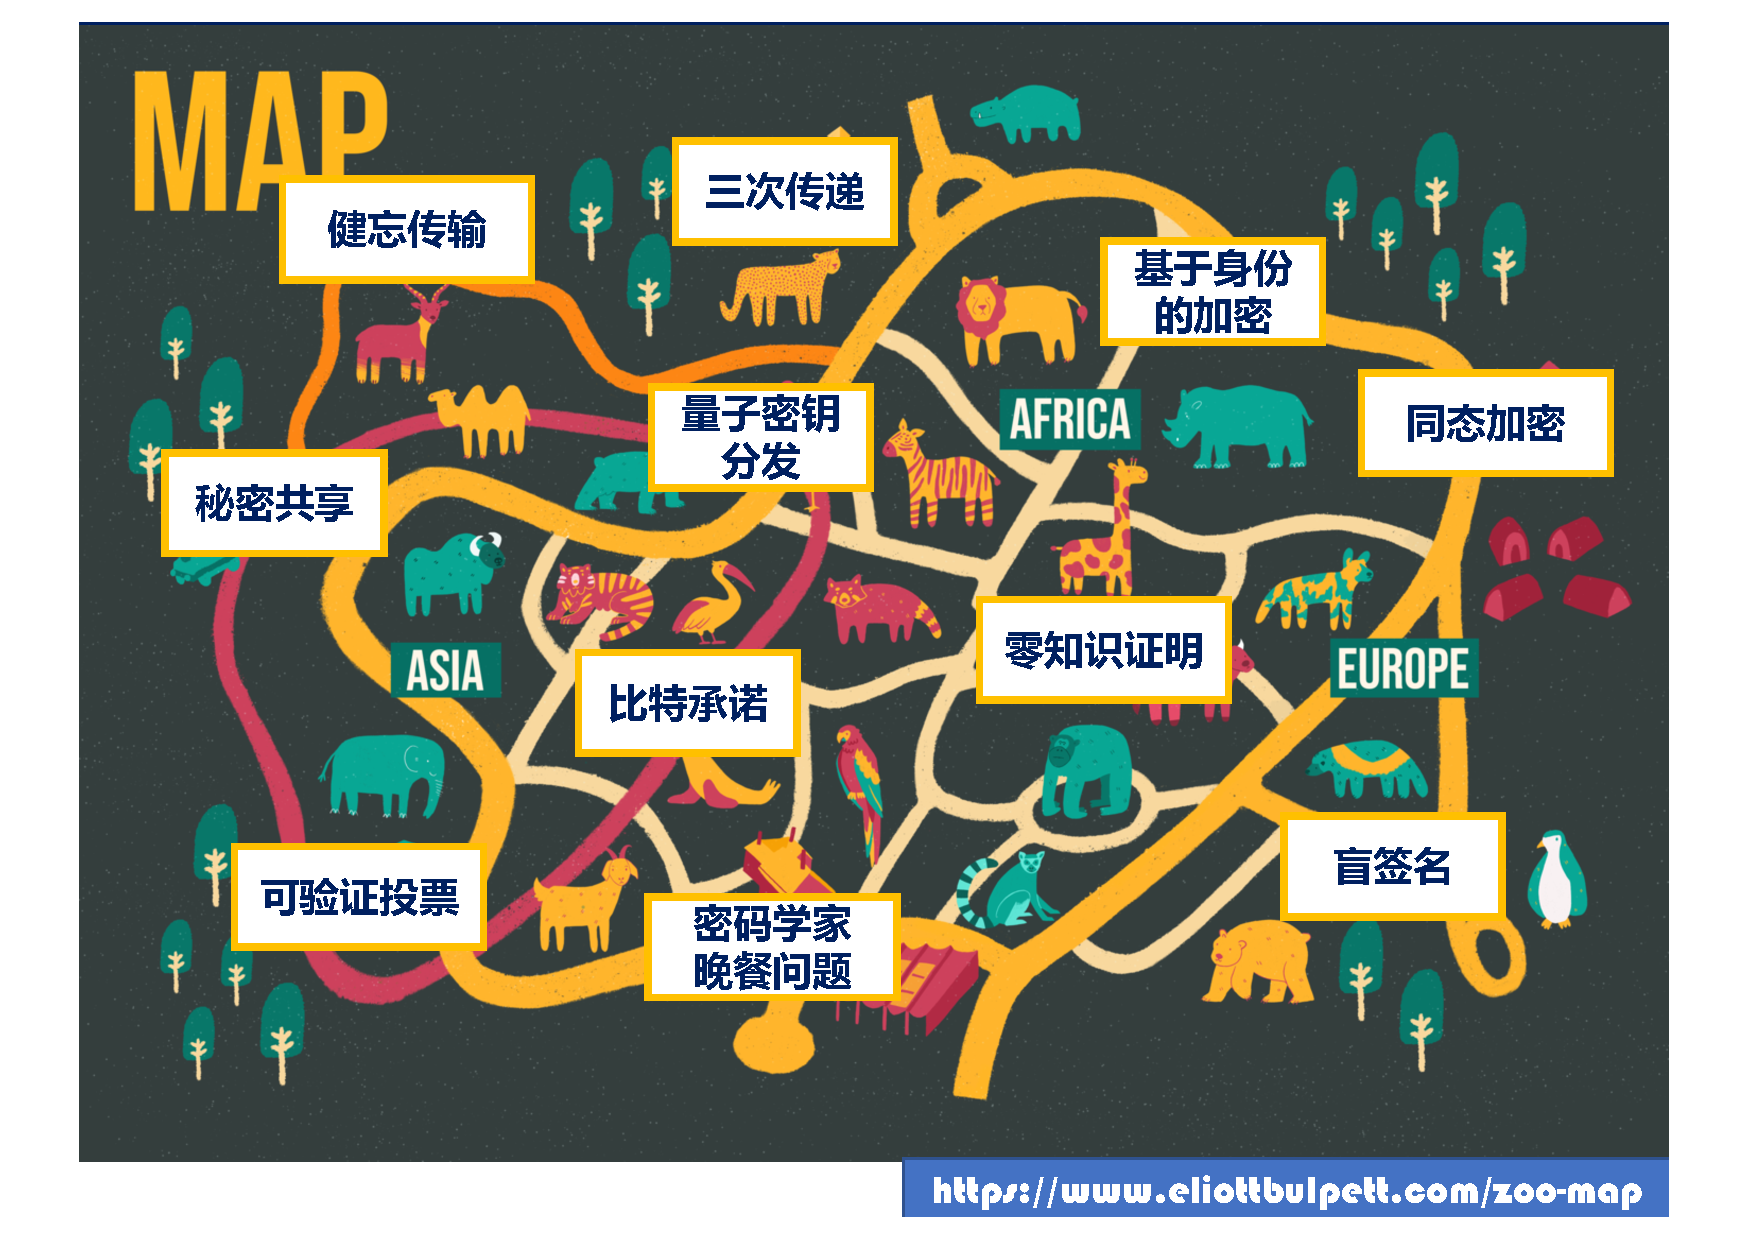
\includegraphics[width=105mm]{pic/zoo-cn.pdf} 
\end{center}
\end{figure}
\end{frame}
\begin{frame}
\frametitle{Outline}
\tableofcontents
\end{frame}
\section{Protocols}
\begin{frame}\frametitle{Protocols (Animals)}
\begin{itemize}
\item \textbf{Communications protocol} is a formal description of digital message formats and the rules for exchanging those messages for a specific purpose.
\begin{itemize}
\item Protocols are to communications what algorithms are to computations
\item Everyone must know it and agree to follow it
\end{itemize}
\item Unambiguous: each step must be well defined and there must be no chance of a misunderstanding
\item Complete: there must be a specified action for every possible situation
\item It should not be possible to do more or learn more than what is specified in the protocol
\end{itemize}
\end{frame}
\begin{frame}\frametitle{Protocol Types}
\begin{itemize}
\item \textbf{Arbitrated protocols}: An arbitrator is a disinterested third party trusted to complete a protocol.
\item \textbf{Adjudicated protocols}: An adjudicator is also a disinterested and trusted third party. Unlike an arbitrator, he is not directly involved in every protocol.
\item \textbf{Self-enforcing protocols}: the best type of protocol. The protocol itself guarantees fairness.
\end{itemize}
\end{frame}
\begin{frame}\frametitle{Attacks against Protocols}
\begin{itemize}
\item \textbf{Passive attacks}: the attacker does not affect the protocol.
\item \textbf{Active attacks}: the attacker alters the protocol to his own advantage.
\end{itemize}
\textbf{Cheater}: the attacker could be one of the parties involved in the protocol.
\begin{itemize}
\item \textbf{Passive cheaters}: follow the protocol, but try to obtain more information than the protocol intends them to.
\item \textbf{Active cheaters}: disrupt the protocol in progress in an attempt to cheat.
\end{itemize}
\end{frame}
\section{SSL/TLS Handshaking}
\begin{frame}\frametitle{Simplified SSL/TLS Handshaking}
\textbf{Purpose}: generate 4 secret keys with authenticated server\\
\textbf{Requirement}: the client has the public key of Trusted Third Party\\
the server has the certificate of its own $pk$ issued by TTP
\begin{figure}
\begin{center}
\begin{tikzpicture}[font=\footnotesize]
%\node (A) at (0,0) {\Lisa(Client)};
%\node (B) [right of = A, node distance = 4cm] {\Left\Bart(Server)};
\node (A) at (0,0) [minimum size=1cm] {}; \Alice{0}{0}{0.4}; \node at (1cm,0) {Client};
\node (B) [right of = A, node distance = 4cm, minimum size=1cm] {}; \Bob{4cm}{0}{0.4}; \node at (5cm,0) {Server};
\node (1a) [below of=A, node distance=0.7cm] {client random $a$};
\node (1b) [below of=B, node distance=0.7cm] {};
\draw[-latex] (1a) -- (1b) node [midway,above] {};
\node (2a) [below of=1a, node distance=0.5cm] {};
\node (2b) [below of=1b, node distance=0.5cm] {server random $b$};
\draw[-latex] (2b) -- (2a) node [midway,above] {};
\node (3a) [below of=2a, node distance=0.5cm] {};
\node (3b) [below of=2b, node distance=0.5cm] {certificate of $pk$};
\draw[-latex] (3b) -- (3a) node [midway,above] {};
\node (4a) [below of=3a, node distance=0.5cm] {$E_{pk}$(premaster secret $s$)};
\node (4b) [below of=3b, node distance=0.5cm] {};
\draw[-latex] (4a) -- (4b) node [midway,above] {};
\node (5a) [below of=4a, node distance=0.5cm] {Hash of previous msgs};
\node (5b) [below of=4b, node distance=0.5cm] {};
\draw[-latex] (5a) -- (5b) node [midway,above] {};
\node (6a) [below of=5a, node distance=0.5cm] {};
\node (6b) [below of=5b, node distance=0.5cm] {Hash of previous msgs};
\draw[-latex] (6b) -- (6a) node [midway,above] {};
\node (7a) [below of=6a, node distance=0.5cm] {session keys from $(a, b, s)$};
\node (7b) [below of=6b, node distance=0.5cm] {session keys from $(a, b, s)$};
%\draw[-latex] (7b) -- (7a) node [midway,above] {};
%\node (8a) [below of=7a, node distance=0.5cm] {};
%\node (8b) [below of=7b, node distance=0.5cm] {$c_{B2}$};
%\draw[-latex] (8b) -- (8a) node [midway,above] {};
%\node (9a) [below of=8a, node distance=0.5cm] {$c_B = (c_{B1}\| c_{B2})$};
%\node (9b) [below of=8b, node distance=0.5cm] {$c_A = (c_{A1}\| c_{A2})$};
%\node (10a) [below of=9a, node distance=0.5cm] {$m_B = \mathsf{Dec}_{pk_A}(c_B)$};
%\node (10b) [below of=9b, node distance=0.5cm] {$m_A = \mathsf{Dec}_{pk_B}(c_A)$};
\end{tikzpicture}

\end{center}
\end{figure}
\end{frame}
\section{Three-Pass Protocol and Interlock Protocol}
\begin{frame}\frametitle{Three-Pass Protocol}
\textbf{Purpose}: communication without shared keys\\
\textbf{Requirement}: $\mathsf{Dec}_{k_1}(\mathsf{Enc}_{k_2}(\mathsf{Enc}_{k_1}(m))) = \mathsf{Enc}_{k_2}(m)$\\
\textbf{Shamir Protocol}: $p$ is a prime, find $e,d$ with $\gcd(e,p-1)=1$ and $ed \equiv 1 \pmod{p-1}$

\begin{figure}
\begin{center}
\begin{tikzpicture}[font=\footnotesize]
\node (A) at (0,0) [minimum size=1cm] {}; \Alice{0}{0}{0.4};
\node (B) [right of = A, node distance = 4cm, minimum size=1cm] {}; \Bob{4cm}{0}{0.4};
\node (1a) [below of=A, node distance=0.7cm] {$p,e_A,d_A$};
\node (1b) [below of=B, node distance=0.7cm] {$p,e_B,d_B$};
%\draw[-latex] (1a) -- (1b) node [midway,above] {};
\node (2a) [below of=1a, node distance=0.5cm] {$c = [m^{e_A} \bmod p]$};
\node (2b) [below of=1b, node distance=0.5cm] {};
\draw[-latex] (2a) -- (2b) node [midway,above] {};
\node (3a) [below of=2a, node distance=0.5cm] {};
\node (3b) [below of=2b, node distance=0.5cm] {$c_1 = [c^{e_B} \bmod p]$};
\draw[-latex] (3b) -- (3a) node [midway,above] {};
\node (4a) [below of=3a, node distance=0.5cm] {$c_2 = [c_1^{d_A} \bmod p]$};
\node (4b) [below of=3b, node distance=0.5cm] {};
\draw[-latex] (4a) -- (4b) node [midway,above] {};
\node (5a) [below of=4a, node distance=0.5cm] {};
\node (5b) [below of=4b, node distance=0.5cm] {$m=[c_2^{d_B} \bmod p]$};
\end{tikzpicture}

\end{center}
\end{figure}
$c_2^{d_B} = c_1^{d_A\cdot d_B} = c^{e_B\cdot d_A\cdot d_B} = m^{e_A\cdot e_B\cdot d_A\cdot d_B} = m^{e_Ad_A\cdot e_Bd_B} = m$
\textbf{Weakness}: insecurity under the man-in-the-middle attack
\end{frame}
\begin{frame}\frametitle{The Man-In-The-Middle Attack}
Also called \textbf{bucket-brigade attack}: A form of active eavesdropping in which the attacker makes independent connections with the victims and relays messages between them, making them believe that they are talking directly to each other
\begin{figure}
\begin{center}
\begin{tikzpicture}[font=\footnotesize]
\node (A) at (0,0) [minimum size=1cm] {}; \Alice{0}{0}{0.4};
\node (B) [right of = A, node distance = 7cm, minimum size=1cm] {}; \Bob{7cm}{0}{0.4};
\node (E) [right of = A, node distance = 3.5cm] {}; \Evil{3.5cm}{0}{0.4};
\node (1a) [below of=A, node distance=1cm] {$pk_A$};
\node (1e) [below of=E, node distance=1cm] {$pk_E$};
\node (1b) [below of=B, node distance=1cm] {};
\draw[-latex] (1a) -- (1e) -- (1b) node [midway,above] {};
\node (2a) [below of=1a, node distance=0.5cm] {};
\node (2b) [below of=1b, node distance=0.5cm] {$pk_B$};
\node (2e) [below of=1e, node distance=0.5cm] {$pk_E$};
\draw[-latex] (2b) -- (2e) -- (2a) node [midway,above] {};
\node (4a) [below of=2a, node distance=0.5cm] {$c_A = \mathsf{Enc}_{pk_E}(m_A)$};
\node (4b) [below of=2b, node distance=0.5cm] {$c_B = \mathsf{Enc}_{pk_E}(m_B)$};
\node (4e) [below of=2e, node distance=0.5cm] {};
\node (5a) [below of=4a, node distance=0.5cm] {$c_{A}$};
\node (5b) [below of=4b, node distance=0.5cm] {};
\node (5e) [below of=4e, node distance=0.5cm] {$ \mathsf{Enc}_{pk_B}(\mathsf{Dec}_{sk_E}(c_A))$};
\draw[-latex] (5a) -- (5e) -- (5b) node [midway,above] {};
\node (6a) [below of=5a, node distance=0.5cm] {};
\node (6b) [below of=5b, node distance=0.5cm] {$c_{B}$};
\node (6e) [below of=5e, node distance=0.5cm] {$ \mathsf{Enc}_{pk_A}(\mathsf{Dec}_{sk_E}(c_B))$};
\draw[-latex] (6b) -- (6e) -- (6a) node [midway,above] {};
%\node (9a) [below of=6a, node distance=0.5cm] {$c_B = (c_{B1}\| c_{B2})$};
%\node (9b) [below of=6b, node distance=0.5cm] {$c_A = (c_{A1}\| c_{A2})$};
\node (10a) [below of=6a, node distance=0.5cm] {$m_B = \mathsf{Dec}_{pk_A}(c_B)$};
\node (10b) [below of=6b, node distance=0.5cm] {$m_A = \mathsf{Dec}_{pk_B}(c_A)$};
\node (11) at (3.5cm,-1.5cm) [minimum height=4.5cm, minimum width=3.5cm, dotted, draw,rounded corners=1ex] {};
\end{tikzpicture}

\end{center}
\end{figure}
\end{frame}
\begin{frame}\frametitle{Interlock Protocol}
\textbf{Purpose}: foil the man-in-the-middle attack.
\begin{figure}
\begin{center}
\begin{tikzpicture}[font=\footnotesize]
\node (A) at (0,0) [minimum size=1cm] {}; \Alice{0}{0}{0.4};
\node (B) [right of = A, node distance = 4cm, minimum size=1cm] {}; \Bob{4cm}{0}{0.4};
\node (1a) [below of=A, node distance=0.7cm] {$pk_A$};
\node (1b) [below of=B, node distance=0.7cm] {};
\draw[-latex] (1a) -- (1b) node [midway,above] {};
\node (2a) [below of=1a, node distance=0.5cm] {};
\node (2b) [below of=1b, node distance=0.5cm] {$pk_B$};
\draw[-latex] (2b) -- (2a) node [midway,above] {};
\node (3a) [below of=2a, node distance=0.5cm] {$c_A = \mathsf{Enc}_{pk_B}(m_A)$};
\node (3b) [below of=2b, node distance=0.5cm] {$c_B = \mathsf{Enc}_{pk_A}(m_B)$};
\node (4a) [below of=3a, node distance=0.5cm] {$(c_{A1}\| c_{A2})=c_A$};
\node (4b) [below of=3b, node distance=0.5cm] {$(c_{B1}\| c_{B2})=c_B$};
\node (5a) [below of=4a, node distance=0.5cm] {$c_{A1}$};
\node (5b) [below of=4b, node distance=0.5cm] {};
\draw[-latex] (5a) -- (5b) node [midway,above] {};
\node (6a) [below of=5a, node distance=0.5cm] {};
\node (6b) [below of=5b, node distance=0.5cm] {$c_{B1}$};
\draw[-latex] (6b) -- (6a) node [midway,above] {};
\node (7a) [below of=6a, node distance=0.5cm] {$c_{A2}$};
\node (7b) [below of=6b, node distance=0.5cm] {};
\draw[-latex] (7a) -- (7b) node [midway,above] {};
\node (8a) [below of=7a, node distance=0.5cm] {};
\node (8b) [below of=7b, node distance=0.5cm] {$c_{B2}$};
\draw[-latex] (8b) -- (8a) node [midway,above] {};
\node (9a) [below of=8a, node distance=0.5cm] {$c_B = (c_{B1}\| c_{B2})$};
\node (9b) [below of=8b, node distance=0.5cm] {$c_A = (c_{A1}\| c_{A2})$};
\node (10a) [below of=9a, node distance=0.5cm] {$m_B = \mathsf{Dec}_{pk_A}(c_B)$};
\node (10b) [below of=9b, node distance=0.5cm] {$m_A = \mathsf{Dec}_{pk_B}(c_A)$};
\end{tikzpicture}

\end{center}
\end{figure}
\end{frame}
\section{Pairing and Identity-Based Encryption}
\begin{frame}\frametitle{Bilinear Maps}
\begin{itemize}
\item Two cyclic groups: $G_1$ with $+$ and generator $P$, $G_2$ with $\times$.
\item \textbf{Bilinear map} $e: G_1 \times G_1 \to G_2$ with $e(aP, bP)=e(P,P)^{ab}$. 
\item \textbf{Theorem}: When $e$ is efficient, the Decisional Diffie-Helman is easy in $G_1$, as $e(aP, bP) = e(P, P)^{ab} = e(P, abP)$.
\item The Weil and Tate pairings are bilinear maps. $G_1$ is an elliptic-curve group and $G_2$ is a finite field.
\end{itemize}
\begin{figure}
\begin{center}
\begin{tikzpicture}
\node (g1) at (-0.5,0.17) [ellipse,minimum width=4cm,minimum height=1.5cm,draw] {};
\node (g1n) [left of=g1, node distance=2.5cm] {$G_1$};
%\node (p) at (-2,0) [circle, minimum size=0.1cm] {\tiny $P$};
\fill (-2,0) circle (2pt) node (p) [above] {$P$};
\fill (-1,0) circle (2pt) node (abp) [above] {$abP$};

%\node (ap) at (-1,0) [circle,minimum size=0.1cm] {\tiny $aP$};
\fill (0,0) circle (2pt) node (ap) [above] {$aP$};

%\node (bp) at (0,0) [circle, minimum size=0.1cm] {\tiny $bP$};
\fill (1,0) circle (2pt) node (bp) [above] {$bP$};

%\node (abp) at (1,0) [circle, minimum size=0.1cm] {\tiny $abP$};

\node (g2) at (-0.5,-2) [ellipse,minimum width=4cm,minimum height=1cm,draw] {};
\node (g2n) [left of=g2, node distance=2.5cm] {$G_2$};

\fill (-0.5,-1.8) circle (2pt) node (gab) [below] {$e(P,P)^{ab}$};

\filldraw [blue!40] (-1.7,-1.1) rectangle (0.7,-0.7);
\node at (-0.5, -0.9) {mapping $e$};

\node (e1) at (-1.5,-0.9) {};
\draw[-latex,blue] (p) -- (e1);
\draw[-latex,blue] (abp) -- (e1);
\draw[-latex,blue] (e1) -- (gab);

\node (e2) at (0.5,-0.9) {};
\draw[-latex,red] (ap) -- (e2);
\draw[-latex,red] (bp) -- (e2);
\draw[-latex,red] (e2) -- (gab);

%\node (fx) [circle, draw, right of=x, minimum size=1.5cm, node distance=4cm] {$f(x)$};
%\node (hc) at ($(x)+(2cm,-1cm)$) [circle, draw] {$\mathsf{hc}(x)$};
%\node (tp) [draw, right of=x, node distance=2cm] {$\mathsf{tp}$};
%\node (ez) [above of=tp, node distance=0.5cm, blue] {easy};

%\draw[-latex,blue] (x) to [bend left=30,-latex,above] node {easy} (fx);
%\draw[-latex,red] (fx) to [bend left=30,-latex,right] node {hard} (hc);
%\draw[-latex,blue] (x) to [bend right=30,-latex,left] node {easy} (hc);
%\draw[-latex,blue] (fx) -- (tp)  -- (x);
%\draw[-latex,red] (fx) to [bend right=-120,-latex,below] node {hard} (x);
\end{tikzpicture}
\end{center}
\end{figure}
\end{frame}
\begin{frame}\frametitle{Jounx's Key Agreement Protocol}
\begin{figure}
\begin{center}
\begin{tikzpicture}[scale=0.7, every node/.style={scale=0.7}]
\node (A) at (0,0) [minimum size=1.4cm] {}; \Alice{0}{0}{0.4};
\node [below of = A, node distance = 0.7cm] {A};
\node (B) [right of = A, node distance = 4cm, minimum size=1cm] {}; \Bob{4cm}{0}{0.4};
\node [below of = B, node distance = 0.7cm] {B};
\node (C) at (2,3.5) [rounded corners=1ex,minimum size=1cm,label distance=-1cm,label=right:C] {};
\Charlie{2}{3.5}{0.4};
\draw[-latex] (A) -- (B) node [midway,above] {$aP$};
\draw[-latex] (B.190) -- (A.350) node [midway,below] {$bP$};
\draw[-latex] (C.240) -- (A.90)  node [sloped,midway,above] {$cP$};
\draw[-latex] (A.80) -- (C.250)  node [sloped,midway,below] {$aP$};
\draw[-latex] (B.90) -- (C.300)  node [sloped,midway,above] {$bP$};
\draw[-latex] (C.290) -- (B.100) node [sloped,midway,below] {$cP$};
\end{tikzpicture}
\end{center}
\end{figure}
\begin{itemize}
\item Recall Jounx's one-round, 3-party key agreement protocol, where
Alice computes the key $e(bP, cP)^a = e(P, P)^{abc}$.
\item \textbf{Bilinear Diffie-Helman (BDH) Assumption}: computing $e(P, P)^{abc}$ is hard given $\left<P, aP, bP, cP \right>$.
\item \textbf{Theorem}: Given BDH assumption, Jounx's is secure.
\end{itemize}
\end{frame}
\begin{frame}\frametitle{Elliptic Curve Groups}
\textbf{Elliptic curve group}: points with ``addition'' operation.\\
Any \textbf{elliptic curve} is a plane algebraic curve:
\[ y^2 \equiv x^3 + Ax + B \pmod p\]
where $A,B \in \mathbb{Z}_p$ are constants with $4A^3 + 27B^2\not \equiv 0 \pmod p$.
$\hat{E}(\mathbb{Z}_p)$ is the set of pairs $(x,y) \in \mathbb{Z}_p \times \mathbb{Z}_p$:
\[ \hat{E}(\mathbb{Z}_p) \overset{\text{def}}{=} \{(x,y) \mid x,y\in \mathbb{Z}_p \land y^2 \equiv x^3 + Ax + B \pmod p \}\]
$E(\mathbb{Z}_p) \overset{\text{def}}{=} \hat{E}(\mathbb{Z}_p)\cup \{\mathcal{O}\}$, $\mathcal{O}$ is identity, ``\textbf{point at infinity}''.
\end{frame}
\begin{frame}\frametitle{``Addition'' on Points of Elliptic Curves}
\begin{columns}
\begin{column}{5cm}
\begin{figure}
\begin{center}
\begin{tikzpicture}[scale=0.7]

\newcommand*{\ShowIntersection}{
\fill 
    [name intersections={of=ec1 and l1, name=i, total=\t}] 
    [red, opacity=1, every node/.style={above left, black, opacity=1}] 
    \foreach \s in {1,...,\t}{(i-\s) circle (2pt)
        node [above left] {\s}};
}

    \begin{axis}[
            xmin=-4,
            xmax=4,
            ymin=-4,
            ymax=4,
            %grid=both,
            %grid style={line width=.1pt, draw=gray!10},
            %major grid style={line width=.2pt,draw=gray!50},
            %xlabel={$x$},
            %ylabel={$y$},
            %scale only axis,
            xtick=\empty, ytick=\empty,
            axis lines=middle,
            domain=-2.279018:2.6,      
            samples=101,
            smooth,   
            clip=false,
            % use same unit vectors on the axis
            %axis equal image=true,
        ]
    \addplot[name path global=ec1, blue] {sqrt(x^3-3*x+5)};
    \addplot[name path global=ec2, blue] {-sqrt(x^3-3*x+5)};
    \addplot[name path global=l1, domain=-3:3, red] {0.8*x+1.3};
    \addplot[name path global=v1, orange] coordinates {(2.23,-3.8) (2.23,3.8)};
    %\addplot[name path global=t1, brown] coordinates {(-1,2.7) (2.23,3.1)};
    \addplot[name path global=t2, purple,domain=-3:3] {0.1238*x+2.824};
    \addplot[mark=*] coordinates {(2.23,-3.1)} node [below left] {$-P_3$}; 
    \addplot[mark=*] coordinates {(-1.05,2.65)} node [above left] {$P_4$}; 
    %\ShowIntersection;

\fill 
    [name intersections={of=ec1 and l1, by={p2, p3}}] 
    [black, opacity=1]
    (p2) circle (2pt) node [above] {$P_2$}
    (p3) circle (2pt) node [above left] {$P_3$};

\fill 
    [name intersections={of=ec2 and l1, by={p1}}] 
    [opacity=1] 
    (p1) circle (2pt) node [left] {$P_1$};

    %\coordinate[label={10:$P$}] (P) at (axis cs:-1,2.64);
\end{axis}

    %\draw[red,name path=curve2] (-2,-1) -- (2,2);

%    \fill [name intersections={of=ec1 and curve2, by={a,b}}]
%     (a) circle (2pt) node [above left] {$P_3$}
%     (b) circle (2pt) node [above] {$P_2$}
     %(c) circle (2pt) node [left] {$P_1$};

% \draw[dotted,gray,name path=curve3] (1.43,-2) -- (1.43,2);
% \draw[-latex,gray] (-2,0) -- (2,0);
% \draw[-latex,gray] (0,-2) -- (0,2);
% %\draw[blue,name path=curve1] plot[smooth] file {tikz/outfile};
% \draw[red,name path=curve2] (-2,-1) -- (2,2);

% \fill [name intersections={of=curve1 and curve2, by={a,b,c}}]
% (a) circle (2pt) node [above left] {$P_3$}
% (b) circle (2pt) node [above] {$P_2$}
% (c) circle (2pt) node [left] {$P_1$};
% \fill [name intersections={of=curve1 and curve3, by={a,d}}]
% (d) circle (2pt) node [left] {$-P_3$};
% %\fill [name intersections={of=curve1 and curve4, by={a,b}}]
% %(b) circle (2pt) node [left] {$P_4$};
% \node (eq) at (-1,-1.7) {\small $y^2=x^3-x+1$};
% \draw[green] (-2,0.94) node [black,above] {$P_4$} -- (a);
% \draw[fill] (-0.7,1.18) circle (1.5pt);
\end{tikzpicture}
%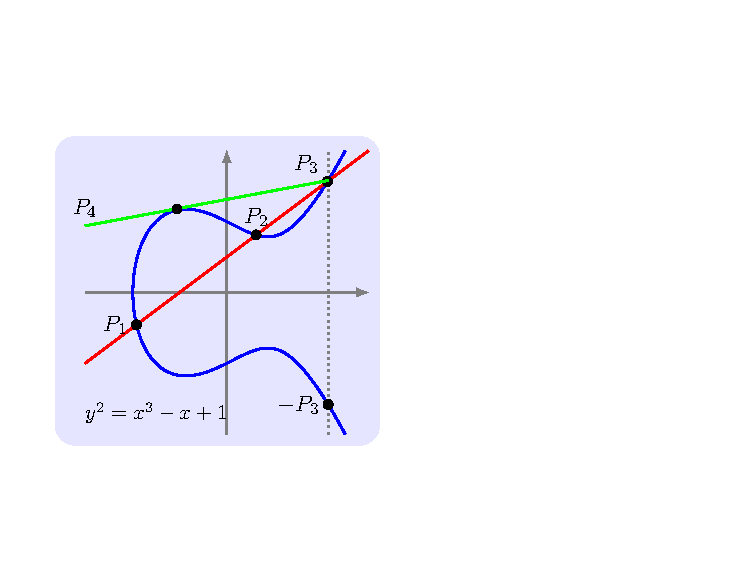
\includegraphics[width=50mm]{pic/ecc.pdf} 
\end{center}
\end{figure}
\end{column}
\begin{column}{5cm}
Every line intersects the curve in 3 points:
\begin{itemize}
\item count twice if tangent.
\item count $\mathcal{O}$ at the vertical infinity of $y$-axis.
\end{itemize}
``\textbf{Addition}'' on points:
\begin{itemize}
\item $P+\mathcal{O} = \mathcal{O} + P = P$.
\item If $P_1, P_2, P_3$ are co-linear, then $P_1 + P_2 + P_3 = \mathcal{O}$.
\end{itemize}
\end{column}
\end{columns}
Some equations: \newline
$-P=(x,-y)$, $P_1 + P_2 = -P_3$, $2P_4=-P_3$, $dP = P + (d-1)P$
\[\text{Key generation:} sk = (P,d); pk = (P,Q=dP)\]
\end{frame}
\begin{frame}\frametitle{Identity-Based Encryption}
\begin{itemize}
\item \textbf{IBE}: Anyone can directly use receiver's ID ($A$) as the pubic key with help of a TTP, aka KGC (Key Generation Center). The receiver obtains its private key from KGC.
\item \textbf{Strength}: TTP could be removed for a finite number of users, no need for PKI.
\item \textbf{Weakness}: Single-point-of-failure, implicit key escrow.
\end{itemize}
\begin{figure}
\begin{center}
\begin{tikzpicture}[font=\footnotesize,scale=0.7, every node/.style={scale=0.7}]
%\node (A) at (0,0) [label=below:Alice] {\Lisa};
%\node (B) [right of = A, node distance = 4cm,label=below:Bob] {\Left\Bart};
\node (A) at (0,0) [minimum size=1cm] {}; \Alice{0}{0}{0.4}; \node at (0,-0.7) {Alice};
\node (B) [right of = A, node distance = 4cm, minimum size=1cm] {}; \Bob{4cm}{0}{0.4}; \node at (4cm,-0.7) {Bob};
\node (KGC) at (2,3) [rounded corners=1ex,minimum width=2cm,draw] {KGC};  
\node at (0,2) [text width=3.6cm, draw, rounded corners=1ex] {generate KGC $pk$ and $sk$; generate Bob's $sk_B$ from $sk$ and "Bob"};
\draw[-latex] (A) -- (B) node [midway,above] {$E_{pk_{B}}(m)$};
%\draw[-latex] (B.70) -- (KGC.350) node [sloped,midway,above] {I want to talk to Bob.};
\draw[-latex] (KGC.340) -- (B.90) node [sloped,midway,below] {$sk_{B}$ for Bob};
\node at (0,-1.5) [text width=3.5cm, draw, rounded corners=1ex] {generate Bob's $pk_{B}$ from KGC's $pk$ and "Bob"};
\end{tikzpicture}
\end{center}
\end{figure}
\end{frame}
\begin{frame}\frametitle{Boneh-Franklin's IBE Scheme}
\textbf{Boneh-Franklin's IBE Scheme} (2001):
\begin{itemize}
\item \textbf{KGC} generates a global public key $pk = sP$ and $sk = s$.
\item \textbf{Encryption}: $\mathsf{Enc}(sP, A, m) = \left< rP, m\oplus H_2(e(H_1(A), sP)^r)\right>$, where $r$ is a random string, $H_1$ and $H_2$ are random oracles.
\item \textbf{Decryption}: The receiver obtains its private key $d_{A} = sH_1(A)$ from KGC. 
 $\mathsf{Dec}(d_{A}, u, v) = v \oplus H_2(e(d_A, u)).$ \\
\item \textbf{Correctness}: $e(d_A, u) = e(sH_1(A), rP) = e(H_1(A), P)^{sr} = e(H_1(A), sP)^r$.
\end{itemize}
\end{frame}
\section{Blind/Group/Ring Signatures}
\begin{frame}\frametitle{Blind Signature}
\textbf{Blind signature} is a form of digital signature in which the message is blinded before it is signed.\\
\textbf{Chaum's blind signature}: Alice asks for Signer to sign $m$ blindly and then sends to Bob
\begin{figure}
\begin{center}
\begin{tikzpicture}[font=\footnotesize]
\node (A) at (0,0) {\Lisa};
\node (r) at (0,-0.7) {a random $r$};
\node (B) [right of = A, node distance = 4cm] {\Left\Bart};
\node (KDC) at (2,3.5) [rounded corners=1ex,minimum width=2cm,label distance=-1.5cm,label=right:Signer] {\Homer};
\node at (3,2.7) {$pk=e$, $sk = d$};  
\draw[-latex] (A) -- (B) node [midway,above] {$s \equiv s'r^{-1}$};
\draw[-latex] (A.90) -- (KDC.240) node [sloped,midway,above] {$m' \equiv mr^e$
};
\draw[-latex] (KDC.250) --  (A.80) node [sloped,midway,below] {$s' \equiv m'^d$};
%\draw[-latex] (KDC.320) to [bend left=40] node [sloped,midway,above] {$\mathsf{cert}_{C\to B}$} (B.70);
%\draw[-latex,dotted] (B.100) -- (KDC.290) node [sloped,midway,below] {Charlie knows $pk_B$.} node [sloped,midway,above] {Bob trusts Charlie.};
\end{tikzpicture}
\end{center}
\end{figure}
\[s \equiv s'r^{-1} \equiv m'^dr^{-1} \equiv (mr^e)^dr^{-1} \equiv m^d.\]
\end{frame}
\begin{frame}\frametitle{Group Signature}
\textbf{Group Signature}: allowing a member of a group to anonymously sign a message on behalf of the group (with a group manager)
\begin{itemize}
\item \textbf{Soundness}: valid sigs by members verify correctly
\item \textbf{Unforaeable}: only members can create valid sigs
\item \textbf{Anonymity}: signer can be determined only by manager
\item \textbf{Traceability}: manager can trace which member signed
\item \textbf{Unlinkability}: cannot tell if two sigs were from same signer
\item \textbf{Exculpability}: cannot forge a sig for other/non members
\end{itemize}
\textbf{A trivial group signature with trusted GM [Chaum (1991)]}:\\
\begin{itemize}
\item \textbf{KeyGen}: GM generates a secret key list for each member and publishes all of public keys
\item \textbf{Sign}: sign with an unused secret key
\item \textbf{Verify}: try all of public keys
\end{itemize}
\end{frame}
%\begin{comment}
\begin{frame}\frametitle{Ring Signature}
\textbf{Ring Signature}: Group signature without group manager, and:
\begin{itemize}
\item cannot revoke the anonymity of an individual signature
\item any group of users can be a group without additional setup
\end{itemize}
\textbf{A ring signature based on bilinear map} [Boneh et al. (2003)]:\\
%$q-$order cyclic groups: $G_1$ with $+$ and generator $P$, $G_2$ with $\times$, bilinear map $e: G_1 \times G_1 \to G_2$ such that $e(aP, bP)=e(P,P)^{ab}$, 
%hash function $H: \{0,1\}^* \to G_1$.
\begin{itemize}
\item \textbf{KeyGen}: for member $U_i$: $sk=x_i \gets Z_q, pk = Y_i = x_iP$.
\item \textbf{Sign}: message $m$ with $(\sigma_i), i=1,\cdots, n$ by $U_k$:
\[\text{for } i\neq k, a_i \gets Z_q, \sigma_i = a_iP;\quad \sigma_k = \frac{1}{x_k}(H(m)-\Sigma_{j\neq k}a_jY_j)\]
\item \textbf{Verify}:
\[ e(H(m),P) = \Pi_ie(Y_i, \sigma_i) \]
\end{itemize}
\end{frame}
%\end{comment}
\section{Secret Sharing/Threshold Crytpography}
\begin{frame}\frametitle{Secret Sharing}
\textbf{Purpose}: distribute a secret amongst a group of $n$ participants, each of whom is allocated a share of the secret. The secret can be reconstructed only when a sufficient number of shares $t$ are combined together. It is called $(t, n)$-\textbf{threshold scheme}.
\newline

\textbf{Blakley's scheme}: any $n$ nonparallel $n$-dimensional hyperplanes intersect at a specific point.

  \begin{minipage}[t]{0.32\linewidth} 
    \centering 
    \includegraphics[width=30mm]{pic/Secretsharing-1} 
  \end{minipage}% 
  \begin{minipage}[t]{0.32\linewidth} 
    \centering 
    \includegraphics[width=30mm]{pic/Secretsharing-2} 
  \end{minipage}
  \begin{minipage}[t]{0.32\linewidth} 
    \centering 
    \includegraphics[width=30mm]{pic/Secretsharing-3}  
  \end{minipage} 

\textbf{Chinese remainder theorem}: the shares of secret are generated by reduction modulo some relatively prime integers, and the secret is recovered by solving the system of congruences using the CRT.
\end{frame}
\begin{frame}\frametitle{Shamir's Secret Sharing}
Adi Shamir ``How to share a secret'', Comm. of ACM, 1979.\\
$t$ points define a polynomial of degree $t-1$, $f(x) = a_0 + a_1x + a_2x^2 + \cdots + a_{t-1}x^{t-1}$, where $a_0$ is the secret $S$, and $a_i$ for $i \neq 0$ is chosen randomly. Choose $n$ points $(x_i, f(x_i))$ for $i = 1, \dots, n$ and send one point to each party.
\begin{exampleblock}{An example of Shamir's secret sharing with $(t=3, n=6)$}
$f(x)= 1234 + 166x + 94x^2 \mod 1613$, where $S = 1234$.\\
6 points: $(1, 1494), (2, 329), (3, 965), (4, 176), (5, 1188), (6, 755)$. \\
Attacker has 2 points $(1, 1494)$ and $(2, 329)$ and try to learn $S$.\\
$1419 = S + a_1 + a_2 - 1613m_1 $, $329 = S + 2a_1 + 4a_2 - 1613m_2$,\\
$448 = a_1 + 3 a_2 + 1613(m_1 - m_2)$, $(m_1-m_2)$ could be any integer.\\
There are infinite possible values of $a_1$ and $a_2$, so that $S$ is secured.
\end{exampleblock}
\textbf{Strength:} information theoretic security, extensible for $n$ 
\textbf{Weakness}: Issue with the verification of correctness of the retrieved shares (verifiable secret sharing).
\end{frame}
\begin{frame}\frametitle{Threshold Cryptography}
\textbf{$(t,n)$-threshold scheme}: at least $t$ of parties can efficiently decrypt/sign the ciphertext, while less than $t$ have no useful information\\

\textbf{Threshold Elgamal Cryptosystem}:
\begin{itemize}
\item \textbf{Key sharing}: $sk = s, pk=h=g^s$. Party $i$ obtains a share $s_i$ with Shamir's scheme  ($(t, n)$-threshold secret sharing) such that $s = \Sigma_i s_i\cdot \lambda_i$ with public info $\lambda_i$ and publishes $h_i = g^{s_i}$
\item \textbf{Enc}: $y \gets \mathbb{Z}_q$, $\left<c_1,c_2\right>=\left<g^y,h^y\cdot m\right>$
\item \textbf{Dec}: Party $i$ outputs $d_i = c_1^{s_i}$ and ZKP of $\log_gh_i = \log_{c_1} d_i$
\[ m = c_2/\Pi_i d_i^{\lambda_i} \]
$c_2/\Pi_i d_i^{\lambda_i} = c_2/\Pi_i c_1^{s_i\cdot \lambda_i} = c_2/c_1^{\Sigma_i s_i\cdot \lambda_i} = c_2/c_1^s=m$
\end{itemize}
\end{frame}
\section{Commitment Scheme}
\begin{frame}\frametitle{Commitment Scheme}
\textbf{Commitment scheme} allows one to commit to a value (which can not be changed later, \textbf{binding}) while keeping it hidden (\textbf{hiding}), with the ability to reveal the committed value
\newline
\textbf{Coin flipping over telephone} [Manuel Blum]:
\begin{figure}
\begin{center}
\begin{tikzpicture}[font=\footnotesize]
\node (A) at (0,0) [minimum size=1cm] {}; \Alice{0}{0}{0.4};
\node (B) [right of = A, node distance = 4cm, minimum size=1cm] {}; \Bob{4cm}{0}{0.4};
\node (0a1) [below of=A, node distance=0.7cm] {$b \gets \{H,T\}$};
\node (0b1) [below of=B, node distance=0.7cm] {};
\node (1a) [below of=0a1, node distance=0.5cm] {$m = b\| r$, $r$ is random};
\node (1b) [below of=0b1, node distance=0.5cm] {};
\node (2a) [below of=1a, node distance=0.5cm] {$h = \mathsf{Hash}(m)$};
\node (2b) [below of=1b, node distance=0.5cm] {};
\draw[-latex] (2a) -- (2b) node [midway,above] {};
\node (3a) [below of=2a, node distance=0.5cm] {};
\node (3b) [below of=2b, node distance=0.5cm] {$b' \in \{H,T\}$};
\draw[-latex] (3b) -- (3a) node [midway,above] {};
\node (4a) [below of=3a, node distance=0.5cm] {$m$};
\node (4b) [below of=3b, node distance=0.5cm] {$h \overset{?}{=} \mathsf{Hash}(m)$};
\draw[-latex] (4a) -- (4b) node [midway,above] {};
\node (5a) [below of=4a, node distance=0.5cm] {};
\node (5b) [below of=4b, node distance=0.5cm] {};
\node (6b) [below of=4b, node distance=0.5cm] {Win if $b=b'$};
\end{tikzpicture}

\end{center}
\end{figure}
\alert{Q1: Is $\mathsf{Hash}$ as CRHF enough for hiding? \\
Q2: Is it possible to achieve info.-theoretically binding and info.-theoretically hiding  at the same time?}
\end{frame}
\section{Zero Knowledge Proofs}
\begin{frame}\frametitle{Zero-Knowledge Proof}
O. Goldreich, S. Micali, A. Wigderson, ``How to Play ANY Mental Game,'' ACM Conference on Theory of Computing, 1987
\begin{itemize}
\item \textbf{Interactive proof system} is an abstract machine that models computation as the exchange of messages between two parties: verifier and prover
\item \textbf{Proof of knowledge}: an interactive proof in which \textbf{prover} succeeds convincing \textbf{verifier} that it knows something
\item \textbf{Zero-knowledge proof (ZKP)}: an interactive proof \emph{without revealing anything other than the veracity of the statement}
\begin{itemize}
\item \textbf{Completeness}: if the statement is true, the honest ``verifier'' will be convinced by an honest prover
\item \textbf{Soundness}: if the statement is false, no cheating prover can convince the honest verifier
\item \textbf{Existence}: If OWF exists, ZKP exists for any NP-set
\end{itemize}
\item \textbf{$\Sigma$-protocol}: ZKP in 3 rounds: announcement (commitment), challenge, and response
\end{itemize}
\end{frame}
\begin{frame}\frametitle{A Toy Example of ZKP}
Alice {\color{red} \LARGE \Ladiesroom} proves to Bob {\color{blue} \LARGE \Gentsroom} that she knows the secret word used to open a magic door in a circular cave.
\begin{figure}
\begin{center}
\input{tikz/zkp}
\end{center}
\end{figure}
\alert{Q: If Alice does not know the secret word, what kind of magic could she master to cheat Bob?}
\end{frame}
\begin{frame}\frametitle{ZKP on Hanmilton Cycle}
ZKP for a solution of Hanmilton Cycle (NPC). [Blum (1986)] \\
\textbf{Prover} relabels the graph (1) randomly, encrypts the randomly relabeld graph (2) with $N + N*(N-1)/2$ boxes (3), and sends them to verifier. \\
\textbf{Verifier} asks only one question: either (a) show the relabelled graph is valid by openning all boxes (3); or (b) show one Hanmilton cycle by openning the boxes on the cycle (4).
\begin{figure}
\begin{center}
\begin{tikzpicture}[scale=0.7, every node/.style={scale=0.7}]
\node (1) at (1,1) [draw,circle] {1};
\node (2) at (1,-0.5)[draw,circle] {2};
\node (3) at ($ (2) ! {1} ! 120 :(1) $) [draw,circle] {3};
\node (4) at ($ (2) ! {1} ! -120 :(1) $) [draw,circle] {4};    
\draw [blue] (1) -- (3) -- (4) -- (2) -- (1) -- (4);

\node at (1,-2.5) {(1) The Graph};

\node (c1) at (5,1) [draw,circle] {3};
\node (c2) at (5,-0.5)[draw,circle] {1};
\node (c3) at ($ (c2) ! {1} ! 120 :(c1) $) [draw,circle] {4};
\node (c4) at ($ (c2) ! {1} ! -120 :(c1) $) [draw,circle] {2};  
\draw [red] (c1) -- (c3) -- (c4) -- (c2) -- (c1);
\draw [blue] (c1) -- (c4);

\node at (5,-2.5) {(2) A Relabeled Graph};

\foreach \x / \y in {1 / 3, 2 / 1, 3 / 4, 4 / 2} {
\node at ($(7.0,2.6) + \x*(0.8,0)$) {\x};
\node at ($(7.0,1.8) + \x*(0.8,0)$) [draw,rectangle,minimum size=0.6cm] {\y};
}

\foreach \x / \y in {1 / 2, 1 / 3, 1 / 4, 2 / 3, 2 / 4, 3 / 4} {
\node at ($(7.8,0.8) + \x*(0,-0.8) $) {\x};
\node at ($(7.0,0.8) + \y*(0.8,0) $) {\y};
\node at ($(7,0.8) + \x*(0,-0.8) + \y*(0.8,0)$) [draw,rectangle,minimum size=0.6cm] {1};
%\node at ($(6.5,0.8) + \x*(0,-0.8)$) {\x};
}
\node at ($(7,0.8) + 1*(0,-0.8) + 4*(0.8,0)$) [draw,rectangle,minimum size=0.6cm,fill=white] {0};


\node at (9.2,-2.5) {(3) Commited Boxes};

\foreach \x / \y in {1 / 2, 1 / 3, 1 / 4, 2 / 3, 2 / 4, 3 / 4} {
\node at ($(11.8,0.8) + \x*(0,-0.8) $) {\x};
\node at ($(11.0,0.8) + \y*(0.8,0) $) {\y};
\node at ($(11,0.8) + \x*(0,-0.8) + \y*(0.8,0)$) [draw,rectangle,minimum size=0.6cm] {1};
%\node at ($(6.5,0.8) + \x*(0,-0.8)$) {\x};
}
\node at ($(11,0.8) + 1*(0,-0.8) + 4*(0.8,0)$) [draw,rectangle,minimum size=0.6cm,fill=white] {};
\node at ($(11,0.8) + 2*(0,-0.8) + 3*(0.8,0)$) [draw,rectangle,minimum size=0.6cm,fill=white] {};

\node at (13.2,-2.5) {(4) Opened Boxes};

\end{tikzpicture}
\end{center}
\end{figure}
\end{frame}
\begin{frame}\frametitle{ZKP and Commitment}
The simulation paradigm: by seeing Y , a party learns no more than X if Y can be efficiently generated given only X.\\
A simple example: without commitment, the verifier learns the message given a ciphertext. With commitment, the prover can check whether the verifier already knows the message.
\begin{figure}
\begin{center}
\begin{tikzpicture}[font=\footnotesize]
\node (A) at (0,0) {\Lisa};
\node (B) [right of = A, node distance = 4cm] {\Left\Bart};
\node (0a1) [below of=A, node distance=1cm] {Prover knows $sk$};
\node (0b1) [below of=B, node distance=1cm] {a random $m$};
\node (0a) [below of=0a1, node distance=0.5cm] {$m' = \mathsf{Dec}_{sk}(c)$};
\node (0b) [below of=0b1, node distance=0.5cm] {$c \gets \mathsf{Enc}_{pk}(m)$};
\draw[-latex] (0b) -- (0a) node [midway,above] {$c$};
\node (1a) [below of=0a, node distance=0.5cm] {};
\node (1b) [below of=0b, node distance=0.5cm] {};
%\draw[-latex] (1a) -- (1b) node [midway,above] {};
\node (2a) [below of=0a, node distance=1cm] {$h = \mathsf{commit}(m')$};
\node (2b) [below of=0b, node distance=1cm] {};
\draw[-latex] (2a) -- (2b) node [midway,above] {$h$};
\node (3a) [below of=2a, node distance=0.5cm] {$m \overset{?}{=} m'$};
\node (3b) [below of=2b, node distance=0.5cm] {};
\draw[-latex] (3b) -- (3a) node [midway,above] {$m$};
\node (4a) [below of=3a, node distance=0.5cm] {If No, stop;};
\node (4b) [below of=3b, node distance=0.5cm] {};
\node (5a) [below of=4a, node distance=1cm] {};
\node (5b) [below of=4b, node distance=1cm] {Accept if $m=m'$};
\draw[-latex] (5a) -- (5b) node [midway,above] {$m'$};
\node (6b) [below of=5b, node distance=0.5cm] {};
\node (11) at (1.5cm,-3cm) [minimum height=2cm, minimum width=6cm, dotted, draw,rounded corners=1ex] {};
\end{tikzpicture}

\end{center}
\end{figure}
\end{frame}
\begin{frame}\frametitle{Schnorr Protocol}
We have learned a ZKP as an identification scheme. Recall \textbf{Schnorr protocol}: Alice proves to Bob the knowledge of $x=\log_gy$ in the discrete log problem.
\begin{figure}
\begin{center}
\begin{tikzpicture}[font=\footnotesize]
\node (A) at (0,0) [minimum size=1cm] {}; \Alice{0}{0}{0.4};
\node (B) [right of = A, node distance = 4cm, minimum size=1cm] {}; \Bob{4cm}{0}{0.4};
\node (0a) [below of=A, node distance=0.7cm] {a random $r$};
\node (0b) [below of=B, node distance=0.7cm] {};
\node (1a) [below of=0a, node distance=0.5cm] {$t = g^r$};
\node (1b) [below of=0b, node distance=0.5cm] {};
\draw[-latex] (1a) -- (1b) node [midway,above] {};
\node (2a) [below of=1a, node distance=0.5cm] {};
\node (2b) [below of=1b, node distance=0.5cm] {a random bit $c \gets\{0,1\}$};
\draw[-latex] (2b) -- (2a) node [midway,above] {};
\node (3a) [below of=2a, node distance=0.5cm] {$s = r + cx$};
\node (3b) [below of=2b, node distance=0.5cm] {};
\draw[-latex] (3a) -- (3b) node [midway,above] {};
\node (4a) [below of=3a, node distance=0.5cm] {};
\node (4b) [below of=3b, node distance=0.5cm] {$g^s \overset{?}{=} ty^c$};
\end{tikzpicture}

\end{center}
\end{figure}
If Alice can foresee $c$, Alice can cheat with $t=g^s/y$ when $c=1$.
\end{frame}
\begin{frame}\frametitle{ZKP of the Ability to Break RSA}
\textbf{Purpose}: Alice convinces Bob that she knows Charlie's private key $d$ for RSA problem $\langle N,e,d \rangle$, but she doesn't want to tell Bob $d$
\begin{figure}
\begin{center}
\begin{tikzpicture}[font=\footnotesize]
\node (A) at (0,0) [minimum size=1cm] {}; \Alice{0}{0}{0.4};
\node (B) [right of = A, node distance = 4cm, minimum size=1cm] {}; \Bob{4cm}{0}{0.4};
\node (0a) [below of=A, node distance=0.7cm] {};
\node (0b) [below of=B, node distance=0.7cm] {};
\draw[latex-latex] (0a) -- (0b) node [midway,above] {random $k,s > 3$} node [midway,below] {$ks \equiv e \pmod N$};
\node (1a) [below of=0a, node distance=0.5cm] {};
\node (1b) [below of=0b, node distance=0.5cm] {};
%\draw[-latex] (1a) -- (1b) node [midway,above] {};
\node (2a) [below of=1a, node distance=0.5cm] {};
\node (2b) [below of=1b, node distance=0.5cm] {};
\draw[latex-latex] (2b) -- (2a) node [midway,above] {random $c$};
\node (3a) [below of=2a, node distance=0.5cm] {$m = c^d $};
\node (3b) [below of=2b, node distance=0.5cm] {};
%\draw[-latex] (3a) -- (3b) node [midway,above] {};
\node (4a) [below of=3a, node distance=0.5cm] {$x = m^k $};
\node (4b) [below of=3b, node distance=0.5cm] {};
\draw[-latex] (4a) -- (4b) node [midway,above] {};
\node (5b) [below of=4b, node distance=0.5cm] {$x^s \overset{?}{=} c$};
\end{tikzpicture}

\end{center}
\end{figure}
If Alice can manipulate $c$, Alice can cheat with $c = m^e$.
\end{frame}
\section{Oblivious Transfer}
\begin{frame}\frametitle{Oblivious Transfer}
\textbf{Oblivious transfer (OT)} protocol: a sender remains oblivious as to whether or which info has been transferred. \\
\footnotesize A toy example of \textbf{Socialist Millionaires Problem}: Alice (\$3M) and Bob (\$2M) wonder whether they makes the same money, while keeping their salaries secret. \href{http://twistedoakstudios.com/blog/Post3724_explain-it-like-im-five-the-socialist-millionaire-problem-and-secure-multi-party-computation}{\alert{[source link]}}
\begin{columns}
\begin{column}{6cm}
\begin{figure}
\begin{center}
\begin{tikzpicture}[scale=0.8, every node/.style={scale=0.8}]
\foreach \y in {1, 2, 3, 4} {
\node (r\y) at ($ (0.8cm,0) - \y*(0,1.6cm)$) [fill=blue!10] {\y};
\foreach \x in {1, 2, 3, 4} {
\node (f\y\x) at ($\x*(1.8cm,0) - \y*(0,1.6cm)$) [minimum size=1.2cm,draw] {\$\x M};
\draw ($\x*(1.8cm,0) - \y*(0,1.6cm) + (-0.6cm, 0.6cm)$) -- +(0.3cm,0.2cm) -- +(1.5cm,0.2cm) -- +(1.2cm,0cm);
\draw ($\x*(1.8cm,0) - \y*(0,1.6cm) + (0.9cm, 0.8cm)$) -- +(0cm,-1.2cm) -- +(-0.3cm,-1.4cm);
\draw [blue] ($\x*(1.8cm,0) - \y*(0,1.6cm) + (-0.1cm, 0.7cm)$) -- +(0.4cm,0cm);
\filldraw [blue] ($\x*(1.8cm,0) - \y*(0,1.6cm) + (0.45cm, 0.1cm)$) circle (0.05cm) -- +(0cm,-0.3cm);

%\node (m\y\x) [above of=f\y\x, node distance=2cm] {$m_\x$};
%\node (c\y\x) [below of=f\y\x, node distance=2cm] {$c_\x$};
%\draw[-latex] (m\x) -- (f\x);
%\draw[-latex] (f\x) -- (c\x);
} }

\foreach \y in {2, 3, 4} {
\foreach \x in {1, 3, 4} {
\filldraw [red] ($\x*(1.8cm,0) - \y*(0,1.6cm) + (0.4cm, -0.2cm)$) rectangle +(0.1cm, .5cm]);
} }

\foreach \x in {1, 2, 4} {
\node (yn\x) at ($\x*(1.8cm,0) - 3*(0,1.6cm) + (0.1cm,0.6cm)$) [fill=blue!20,rotate=45,draw] {\footnotesize NO};
}

\node (yn3) at ($3*(1.8cm,0) - 3*(0,1.6cm) + (0.1cm,0.6cm)$) [fill=blue!20,rotate=45,draw] {\footnotesize YES};

%\foreach \x in {1, 3, 4} {
%\node (yn\x) at ($\x*(1.8cm,0) - 3*(0,1.6cm) + (0.1cm,0.6cm)$) [fill=blue!20, minimal size=1.2cm, draw] {};
%}

\node (yn3) at ($2*(1.8cm,0) - 4*(0,1.6cm) + (0.1cm,0.6cm)$) [fill=blue!20,rotate=45,draw] {\footnotesize NO};

\end{tikzpicture}

\end{center}
\end{figure}
\end{column}
\begin{column}{6cm}
\footnotesize
\begin{enumerate}
\item Bob prepares 4 lockable suggestion boxes marked w/ salaries.
\item Bob destroys the keys except for the box marked w/ his salary.
\item Alice puts a paper ``YES'' into the box marked w/ her salary, ``NO'' for the others.
\item Bob open the box and may (or may not) share the paper with Alice.
\end{enumerate}
\end{column}
\end{columns}
\alert{Alice sends 4 papers to Bob, but is oblivious to which paper Bob gets.}
\end{frame}
\begin{frame}\frametitle{Rabin's OT Protocol}
\textbf{Rabin's OT protocol}: Alice is not sure about whether Bob receives the message. RSA problem $\langle N, e, d\rangle $.
\begin{figure}
\begin{center}
\begin{tikzpicture}[font=\footnotesize]
\node (A) at (0,0) {\Lisa};
\node (B) [right of = A, node distance = 4cm] {\Left\Bart};
\node (0a) [below of=A, node distance=1cm] {$N, e, m^e \bmod N$};
\node (0b) [below of=B, node distance=1cm] {};
\draw[-latex] (0a) -- (0b) node [midway,above] {};
\node (1a) [below of=0a, node distance=0.5cm] {};
\node (1b) [below of=0b, node distance=0.5cm] {a random $x$};
%\draw[-latex] (1a) -- (1b) node [midway,above] {};
\node (2a) [below of=1a, node distance=0.5cm] {};
\node (2b) [below of=1b, node distance=0.5cm] {$x^2 \bmod N$};
\draw[-latex] (2b) -- (2a) node [midway,above] {};
\node (3a) [below of=2a, node distance=0.5cm] {the square root $y$ of $x^2$};
\node (3b) [below of=2b, node distance=0.5cm] {};
\draw[-latex] (3a) -- (3b) node [midway,above] {};
\node (4a) [below of=3a, node distance=0.5cm] {};
\node (4b) [below of=3b, node distance=0.5cm] {learn $m$ if $y \neq \pm x$};
\end{tikzpicture}

\end{center}
\end{figure}
If $y \neq \pm x$, then Bob can factorize $N$ with $\gcd(y-x,N)$ and find $d$. Since every quadratic residue modulo $N$ has four square roots, Bob can learn $m$ with probability $\frac{1}{2}$.
\end{frame}
\begin{frame}\frametitle{1-out-of-2 Oblivious Transfer}
\textbf{1-out-of-2 OT}: the sender has two messages $m_0$ and $m_1$, and the receiver  wishes to receive $m_b$, without the sender learning $b$, while the sender ensures that the receiver receive only one message. \\
\textbf{Privacy}: What is retrieved by the receiver is protected, while the sender only reveals one of two messages.
\begin{figure}
\begin{center}
\begin{tikzpicture}[font=\footnotesize]
\node (A) at (0,0) [minimum size=1cm] {}; \Alice{0}{0}{0.4};
\node (B) [right of = A, node distance = 4cm, minimum size=1cm] {}; \Bob{4cm}{0}{0.4};
\node (0a1) [below of=A, node distance=1cm] {RSA: $N,e$};
\node (0b1) [below of=B, node distance=1cm] {};
\draw[-latex] (0a1) -- (0b1) node [midway,above] {};
\node (0a) [below of=0a1, node distance=0.5cm] {random $x_0,x_1$};
\node (0b) [below of=0b1, node distance=0.5cm] {};
\draw[-latex] (0a) -- (0b) node [midway,above] {};
\node (1a) [below of=0a, node distance=0.5cm] {};
\node (1b) [below of=0b, node distance=0.5cm] {pick $b$, random $k$};
%\draw[-latex] (1a) -- (1b) node [midway,above] {};
\node (2a) [below of=1a, node distance=0.5cm] {};
\node (2b) [below of=1b, node distance=0.5cm] {$v = x_b+k^e$};
\draw[-latex] (2b) -- (2a) node [midway,above] {};
\node (3a) [below of=2a, node distance=0.5cm] {$k_0 = (v - x_0)^d$, $k_1 = (v - x_1)^d$};
\node (3b) [below of=2b, node distance=0.5cm] {};
%\draw[-latex] (3a) -- (3b) node [midway,above] {};
\node (4a) [below of=3a, node distance=0.5cm] {$m_0'= m_0+k_0, m_1'= m_1+k_1$};
\node (4b) [below of=3b, node distance=0.5cm] {};
\draw[-latex] (4a) -- (4b) node [midway,above] {};
\node (5a) [below of=4a, node distance=0.5cm] {};
\node (5b) [below of=4b, node distance=0.5cm] {$m_b = m_b' - k$};
%\node (6b) [below of=5b, node distance=0.5cm] {Win if $b=b'$};
\end{tikzpicture}

\end{center}
\end{figure}
\end{frame}
\section{Secure Multi-Party Computation and Homomorphic Enc.}
\begin{frame}\frametitle{Secure Multi-Party Computation}
\textbf{Secure multi-party computation (MPC)}: enable parties to jointly compute a function over their inputs, while at the same time keeping these inputs private\\
\textbf{Dining Cryptographers Problem}: how to perform a secure MPC of the boolean-OR function [David Chaum (1988)]
\begin{columns}
\begin{column}{4cm}
\begin{figure}
\begin{center}
\input{tikz/dining}
\end{center}
\end{figure}
\end{column}
\begin{column}{6cm}
\begin{itemize}
\item at most one {\color{red} \LARGE \Gentsroom} (1), other {\color{blue} \LARGE \Gentsroom} (0)
\item every two adjacent people establish a shared one-bit secret
\item everyone shouts the XOR of two shared secrets and its own bit
\item output the XOR of all of what everyone shouts. If $1$, there is a {\color{red} \LARGE \Gentsroom}, otherwise there is none
\end{itemize}
\end{column}
\end{columns}
\end{frame}
\begin{frame}\frametitle{Homomorphic Encryption}
\begin{itemize}
\item \textbf{Homomorphic Encryption} with $\circ$: $\mathsf{Dec}_{sk}(c_1\circ c_2)=m_1\circ m_2$.
\item Elgamal encryption is homomorphic with $\times$: $\left<g^{y_1},h^{y_1}\cdot m_1\right>\cdot \left<g^{y_2},h^{y_2}\cdot m_2\right> = \left<g^{y_1+y_2},h^{y_1+y_2}\cdot m_1m_2\right>$
\item Paillier scheme is homomorphic with $+$: $\mathsf{Enc}_N(m_1) \cdot \mathsf{Enc}_N(m_2) = \mathsf{Enc}_N([m_1+m_2 \bmod N])$.
\item \textbf{Application}: voting without learning any individual votes.
\[c_i := [(1+N)^{v_i}\cdot r^N \bmod N^2], v_i \in \{0,1\}\]
\[c^* := [\Pi_{i} c_i \bmod N^2], v^* = \Sigma_{i} v_i \]
\item First \textbf{Fully} homomorphic with $\times$ and $+$ by Craig Gentry (2009).
\end{itemize}
\end{frame}
\section{End-to-End Voting}
\begin{frame}\frametitle{End-to-End Voting System}
\textbf{End-to-End Voting System}:
\begin{enumerate}
\item \textbf{Cast}: Voter casts ballot at Voting Machine (VM) %, and gets a copy as ``receipt''
\item \textbf{Post}: Ballots are posted on Public Bulletin Board (PBB)
\item \textbf{Count}: Tally is computed by election officials (EO) from PBB
\end{enumerate}
\textbf{Security goals}:
\begin{itemize}
\item \textbf{End-to-End Verifiability}: any voter gets assurance that \textbf{cast as intended}, \textbf{post as cast}, and \textbf{counted as posted};
\item \textbf{Privacy}: no one knows what the voter cast; even the voter can not convince others what she cast; privacy also means \textbf{coercion-resistance};
\end{itemize}
\end{frame}
\begin{frame}\frametitle{ThreeBallot [Rivest (2006)] w/o Crypto}
Philosophy: "vote by rows, cast by columns"
\begin{figure}
\begin{center}
\begin{tikzpicture}[scale=0.7, every node/.style={scale=0.7}]
\foreach \n in {0, 1} {
\foreach \x in {1, 2, 3} {
\node (f\n\x) at ($\x*(2cm,0) + \n*(7cm,0)$) [minimum width=2cm, minimum height=2.5cm, align=left, draw] {Alice\\ Bob\\ Charlie\\[2ex] ID\pgfmathparse{random(1000,9000)}\pgfmathresult};
	\foreach \y in {1, 2, 3} {
	\filldraw [draw=black,fill=white] ($\x*(2cm,0) + (0.7cm,1.4cm) - \y*(0,0.5cm) + \n*(7cm,0)$) circle (4pt);
	}
} }
\filldraw [black] ($3*(2cm,0) + (0.7cm,1.4cm) - 1*(0,0.5cm) + 1*(7cm,0)$) circle (4pt);
\filldraw [black] ($1*(2cm,0) + (0.7cm,1.4cm) - 2*(0,0.5cm) + 1*(7cm,0)$) circle (4pt);
\filldraw [black] ($2*(2cm,0) + (0.7cm,1.4cm) - 2*(0,0.5cm) + 1*(7cm,0)$) circle (4pt);
\filldraw [black] ($2*(2cm,0) + (0.7cm,1.4cm) - 3*(0,0.5cm) + 1*(7cm,0)$) circle (4pt);
\node [below of=f02, node distance=1.6cm] {Empty ballots};
\node [below of=f12, node distance=1.6cm] {Vote for Bob};
\end{tikzpicture}

\end{center}
\end{figure}
\begin{itemize}
\item Each voter casts three plaintext ballots.
\item Each row has 1 or 2 marks. Not 0, not 3.
\item Each ballot should have a unique ID.
\item All three cast ballots go on PBB.
\item Voter takes home copy of arbitrarily-chosen one as receipt.
\item Receipt serves as integrity check on PBB.
\item \alert{Does threeballot achieve e2e verifiability and privacy?}
\end{itemize}
\end{frame}
\section{Quantum Cryptography}
\begin{frame}\frametitle{Why Quantum Cryptography?}
Quantum cryptography taps the natural uncertainty of the quantum world
\begin{itemize}
\item \textbf{Superposition}: object doesn't have definite properties (location, speed) but has probabilities over them
\item \textbf{Interference}: probabilities can be negative
\item \textbf{Entanglement}: properties of many particles can be correlated
\item \textbf{Measurement}: object's properties collapse to definite value when measured, collapsing also properties of other entangled objects
\end{itemize}
\end{frame}
\begin{frame}\frametitle{State-of-the-Art of Quantum Cryptography}
\begin{itemize}
\item (Unsurprisingly) there is \textbf{no proof} that quantum computers are more powerful than classical computers/Boolean circuits/Turing machines
\item There are \textbf{polynomial} algorithms (e.g., Shor's algorithm) for quantum computers solving problems unknown to be solvable classically in poly-time: factoring and discrete logs
\item There are \textbf{hard} problem with no quantum poly-time algorithm: NPC, inverting many candidate OWF, private key encryption and signature schemes
\end{itemize}
\end{frame}
\begin{frame}[fragile]\frametitle{Quantum Key Distribution}
\textbf{Purpose}: Using photon polarization states to transmit the information in a public channel against eavesdroppers

\begin{exampleblock}{BB84 protocol: C. H. Bennett and G. Brassard (1984)}
{\centering	
\begin{tabular}{|c|c|c|} \hline
Basis & \verb#0# & \verb#1# \\ \hline
\verb#+# & \verb#|# & \verb#-# \\ \hline
\verb#x# & \verb#/# & \verb#\# \\ \hline
\end{tabular}	
\begin{tabular}{|r|c|} \hline
Alice's random bits & \verb#01101001# \\ \hline
Alice's random sending basis & \verb#++x+xxx+# \\ \hline
Photon polarization Alice sends & \verb#|-\|\//-# \\ \hline
Bob's random measuring basis & \verb#+xxx+x++# \\ \hline
Photon polarization Bob measures & \verb#|/\/-/--# \\ \hline
Shared secret key & \verb#0 1  0 1# \\ \hline
\end{tabular}
}
\begin{itemize}
\item Two bases are public
\item Eavesdropping would change the photon polarization states
\item Check for the presence of eavesdropping by comparing a subset of shared bit string
\end{itemize}
\end{exampleblock}
\end{frame}

\begin{frame}\frametitle{Summary}
One of Clarke’s three laws: \it{Any sufficiently advanced technology is indistinguishable from magic.}

\end{frame}
\end{document}
